%!TEX TS-program = xelatex
%!TEX encoding = UTF-8 Unicode

\documentclass{harvard-thesis}
%\usepackage[spanish]{babel}
%\selectlanguage{spanish}
%\usepackage[utf8x]{inputenc}
\usepackage{alltt}
\usepackage{mdframed}
\begin{document}
\pagenumbering{gobble}
%%%%%%%%% Para el codigo .feature %%%%%%%%%%
\newcommand{\feature}[1]{\textcolor[rgb]{0.0,0.35,0.6}{#1}}
\newcommand{\ftable}[1]{\color{orange}}
\newcommand{\bgcode}[1]{\color[rgb]{0.93,0.93,0.93}}
\definecolor{bgcode}{rgb}{0.95,0.95,0.95}

%%%%%%%%%%%%%%% %para cambiar la fuente en secciones solamente %%%%%%%%%%%%%%%
%http://tex.stackexchange.com/questions/25249/how-do-i-use-a-particular-font-for-a-small-section-of-text-in-my-document
%\renewcommand{\sfdefault}{phv}
%{\setmonofont{Monaco} texto ....}
%\fontfamily{Monaco}\selectfont
%\newcommand*{\myfontcmd}{\fontfamily{phv}\selectfont}
%\newenvironment{myfont}{\fontfamily{phv}\selectfont}{\par}
%%%%%%%%%%%%%%%%%%%%%%%%%%%%%%%%%%%%%%%%%%%%%%%%%%%%%%%%%%%%%%%%%%%%%%%%%%%%%

\lstdefinelanguage{Feature} {
    morekeywords={
        Característica, Como, Quiero, Para, Esquema del escenario,
        Dado, Y, Cuando, Entonces, Pero, Feature, As, In order to,
        I want, Scenario, Given, And, When, Then, But,
        },
    sensitive=false,
    morecomment=[s]{<}{>},
    alsoletter={:}
}

\lstset{
  framesep=5pt,
  backgroundcolor=\color[rgb]{0.93,0.93,0.93},
  basicstyle=\scriptsize,
  showstringspaces=false,
  %breaklines=true,
  %%%%%%%%%%%%%
  keywordstyle=\feature,
  identifierstyle=\ttfamily,
  stringstyle=\ttfamily\color{orange},
  commentstyle=\color{orange},
  %%%%%%%%%%%%%
  %keywordstyle={\bfseries \feature},
  %numbers=left, numberstyle=\tiny, stepnumber=2, numbersep=5pt,
%  alsoletter={:,<,>},
  %morekeywords={Característica, Como, Quiero, Para, Esquema del escenario, Dado, Y, Cuando, Entoces, Pero},
  escapechar=\&% char to escape out of listings and back to LaTeX
  alsoletter={:}
}

%%%%%%%%%%%%%%%%%%%%%%%%%%%%%%%%%%%%%%%%%%%%

% Margenes segun especificion de la UMSS
\marginsize{3cm}{2cm}{1cm}{2cm}

% the front matter
\pagestyle{empty}
% some details about the thesis
\title{SISTEMA DE CONTROL Y SEGUIMIENTO DE VEH\'ICULOS}
\author{P\'EREZ SOTO, Jos\'e Benjam\'in}
\tutor{Lic. LAIME ZAPATA, Valentin}
\advisor{Lic. LAIME ZAPATA, Valentin}

% about the degree
\degree{Licenciatura en Inform\'atica}
\degreeyear{2014}
\degreemonth{Diciembre}

% about the university
\department{INGENIER\'IA INFORM\'ATICA}
\university{UNIVERSIDAD MAYOR DE SAN SIM\'ON}
\facultad{FACULTAD DE CIENCIAS Y TECNOLOG\'IA}
\universitycity{Cochabamba}
\universitystate{Bolivia}

\maketitle
%\copyrightpage
\abstractpage
\tableofcontents
%\authorlist
\listoffigures
%\listoftables
\dedicationpage
\acknowledgments

\onehalfspacing

% incluude each chapter...
%\begin{savequote}[75mm]
%Camina hacia el futuro
%\qauthor{Anonimo}
%\end{savequote}

\chapter{Introducción}

\section{Antecedentes}

\section{Descripción del problema}

\section{Objetivo General}

\section{Objetivos Específicos}

\section{Alcances y Limitaciones}

\subsection{Alcances}

\section{Justificación}


%\begin{savequote}[75mm]
%  El pasado es historia
%\qauthor{Anonimo}
%\end{savequote}

\chapter{Marco Referencial}



%\begin{savequote}[75mm]
%Nulla facilisi. In vel sem. Morbi id urna in diam dignissim feugiat. Proin molestie tortor eu velit. Aliquam erat volutpat. Nullam ultrices, diam tempus vulputate egestas, eros pede varius leo.
%\qauthor{Quoteauthor Lastname}
%\end{savequote}

\chapter{Metodología de Desarrollo para el Sistema}

\newthought{Desarrollo Guiado por Comportamiento} - BDD\footnote{BDD, por sus
siglas en inglés, Behaviour-Driven Development}, es la metodología que se eligió
para el desarrollo del Sistema.

Es una técnica de desarrollo ágil de software que fomenta la colaboración
entre desarrolladores, testers y clientes. Fue nombrado originalmente en el año
2003 por Dan North\footnote{Dan North, \url{http://dannorth.net/} consultado en
fecha 10/06/2014} en respuesta al Desarrollo Guiado por Pruebas - TDD\footnote{TDD,
por sus siglas en inglés, Test-Driven Development}. Podemos considerarlo una evolución
o un mejor entendimiento y una forma mejor de explicar los procesos TDD. Se observo
que los {\it desarrolladores} estaban teniendo momentos difíciles en relación
con TDD que es más una herramienta para diseño que para hacer pruebas.

%en el que el énfasis se pone más en las especificaciones
%finales del software antes que en sus detalles técnicos.

\section{Test-Driven Development - Donde todo empezó}
TDD es una practica de desarrollo que involucra escribir primero los {\it ``Test''}
antes que el código a ser {\it testeado} o probado. Se empieza escribiendo test
muy pequeños para el código que aun no existe, luego de esto si corremos los test
notaremos que los test fallan naturalmente, ahora hay que escribir el código
necesario para que el test pase.

Una vez que pase los tests, observe el diseño resultante, y refactorizar cualquier
duplicación o código innecesario que se encuentre. Es natural que en este momento
el diseño es demasiado simple para manejar todas las responsabilidades que tendrá.

En lugar de añadir mas código, documente la siguiente responsabilidad en el
formulario de los siguientes tests. Ejecútelo, y vea los fallos, escriba el código
necesario para que pase el test, revise el diseño, remueva el código innecesario
o duplicado. Ahora añada el siguiente test, vea los fallos, consiga que pase los
tests, refactorizar, fallo, paso, refactorizar, fallo, paso, refactorizar,
\ldots etc.

\begin{figure}[h]
  \begin{center}
  \includegraphics[width=0.4\textwidth]{figures/chapter2/tdd_cycle.jpg}
  \caption[TDD]{Ciclo del Desarrollo Guiado por Pruebas.}
\end{center}
\end{figure}
En muchos {\it Sistemas de Tests}, cuando un test falla, nosotros vemos los
resultados pintados en {\it rojo}. Después cuando esto pasa, los resultados
son pintados en {\it verde}. Debido a esto, a menudo nos referimos a este ciclo
como {\it rojo/verde/refactorizar}.

\begin{figure}[h]
  \centering
  \includegraphics[width=0.6\textwidth]{figures/chapter2/tdd.png}
  \caption[TDD: red, green, refactor]{Desarrollo Guiado por Pruebas es rojo, verde, refactor.}
\end{figure}

\subsection{Diseño emergente}

Como el código base incrementa en tamaño, encontraron que se da mucha atención
en el paso de refactorización. El diseño esta en constante evolución y bajo
revisión constante, aunque no esta predeterminado. Esto es un {\it diseño
emergente} a un nivel granular y es uno de los subproductos mas significativos
de TDD.

Más que pensar en TDD como una práctica de pruebas, lo vemos como una técnica
utilizada para entregar código de alta calidad a los testers, los que son
responsables de las prácticas de pruebas formales.

Y aquí es donde los {\it Test} en TDD llega a tener problemas. Específicamente,
esta es la idea de {\it unit testing }\footnote{unit testing, son pruebas unitarias}
y esto a menudo conduce a nuevos TDDers para verificar y asegurarse de que un objeto
sea el objeto esperado, como ser un método {\it register()} almacene una colección
de {\it Registers} y sea específicamente un {\it Array}.

Este tipo de detalle en un test crea una dependencia del test en la estructura
interna del objeto que esta siendo probado. Esta dependencia significa, que si
hay otro requerimiento que nos hace cambiar el objeto de Array a Hash el test
fallará, a pesar de que el comportamiento no cambie. Esta fragilidad puede hacer
conjuntos de pruebas mucho mas caras de mantener, y esta es la razón por la que
muchos grupos de pruebas son ignorados o incluso descartados.

En resumen, si estos test internos que se hace a un objeto son contraproducente
a largo plazo, ?`en que debemos centrarnos al escribir estos test por primera vez?

\vspace{0.5cm}
\begin{mdframed}
{\it TDD es una práctica para entregar código de calidad con un buen diseño
  que una práctica para realizar {\bfseries pruebas}}
\end{mdframed}

\section{Behaviour-Driven Development: El siguiente paso}
El problema con los tests que se hacen a la estructura de los objetos es que
estamos probando si {\it es} un objeto en lugar de lo que {\it hace} el objeto. Lo que
{\it hace} un objeto es mucho más importante.

Lo mismo ocurre a nivel de aplicación. Los Stakeholders\footnote{Stakeholders,
los interesadas del sistema} no le dan importancia a que si los datos son
persistentes o no en una base de datos relacional compatible con ANSI. A ellos
les importa de que {\it ``estén en la base de datos''}, por lo general a ellos
les interesa de que este almacenado en {\it algún lugar} de donde ellos puedan
recuperarlo.

\subsection{Todo es Comportamiento}
BDD se enfoca completamente en el {\it comportamiento} en lugar de la estructura,
y lo hace en todos los niveles de desarrollo. Ya sea que estemos hablando de un
objeto que calcule la distancia entre dos ciudades, u otro objeto que delegue la
búsqueda de servicios, o una interfaz de usuario que se provee para hacer feedback
cuando ocurre una salida invalida, {\it todo es comportamiento}.

Una vez que reconocemos esto, cambiamos la forma en que pensamos acerca de la
expulsión de código. Empezamos a pensar mas en la interacción entre las personas
y el sistema, o entre objetos, de los que sabemos acerca de su estructura.

\subsection{Conseguir las Palabras Correctas}
Creemos que la mayoría de los problemas que enfrentan los equipos de desarrollo
de software son los problemas de comunicación. BDD tiene como objetivo ayudar a la
comunicación mediante la simplificación del lenguaje que usamos para describir los
escenarios en los que se utilizara el software: {\it Given} obtener datos de algún
contexto, {\it When} cuando ocurre algún evento, {\it Then} entonces espero algún
resultado.

{\it Given, When, Then}, la triada BDD, son simples palabras que utilizaremos ya
sea que estemos hablando del comportamiento de la aplicación o de un objeto. Estas
palabras son fáciles de entender por los analistas de negocios, testers, y
desarrolladores por igual. Estas palabras están incrustadas en el DSL\footnote{
Domain Specific Language, Lenguaje de dominio especifico} Gherkin.

\subsection{Gherkin}
Gherkin es un DSL legible para gente no técnica, que permite definir el
comportamiento del software sin detallar como está implementado, además de que
nos permite documentar las funcionalidades a la vez que escribimos casos de
prueba automáticos.

Otras ventajas que nos proporciona usar Gherkin:
\begin{itemize}
    \item Fácil de entender
    \item Fácil de leer
    \item Fácil de parsear
    \item Fácil de discutir
\end{itemize}

Gherkin es un lenguaje que usa el indentado para definir la estructura, de manera
que los saltos de linea dividen las diferentes declaraciones, la mayoría de las
lineas empiezan con palabras clave. El parser divide el texto en {\it Features,
Scenarios y Steps}, cuando pasas los casos de prueba, el parser busca un Step con
ese nombre. Los Steps son los análogos de los métodos en Java o las funciones en
Javascript.

La gramática de Gherkin consiste en pocas palabras claves que debe usarse cuando
escribimos un archivo {\it .feature}:

\begin{itemize}
    \item Feature
    \item Background
    \item Scenario
    \item Scenario outline
    \item Examples
    \item Given, When, Then, And, But (Para definir pasos)
    \item | (Para definir tablas)
    \item '''''' (Para definir una cadena de varias lineas)
    \item \# (Para usar comentarios)
\end{itemize}

Se puede escribir lo que uno quiere después de una palabra clave. Las palabras
claves {\it Given, When, Then, And} y {\it But} indican pasos en un escenario, que
usaremos para construir un DSL para un proyecto.

Cada {\it Feature} o {\it característica} se define en un archivo {\it .feature},
un característica normalmente consiste en una serie de {\it escenarios}, el texto
entre {\it Feature} y {\it Scenario} permite definir libremente el contexto ya
que este texto no será usado para ninguna funcionalidad en el código generado,
es meramente descriptivo.

\vspace{0.5cm}
\begin{mdframed}
\begin{alltt}
\emph{Feature:} [nombre de la característica en general a probar]
  \emph{As} [un actor/rol]
  \emph{In order to} [algún beneficio]
  \emph{I want} [una característica]

  \emph{Scenario:} \ldots
\end{alltt}
\end{mdframed}
\vspace{0.5cm}

Nos ayuda a entender {\it como} que tipo de usuario es el que va ha usar esta
característica o funcionalidad, {\it para} que nos sirve esta funcionalidad y que
{\it quiero} obtener.

\subsection{Scenario - Esquema del escenario}
Los escenarios son ejemplos concretos de como queremos que se comporte el software.
Esta manera de hacerlo es mas explicita que algunas formas tradicionales para
describir requerimientos y nos ayudan a plantear y responder preguntas que de lo
contrario no podríamos hacerlas. Los escenarios nos permiten responder a preguntas,
describiendo exactamente lo que debe suceder y en que circunstancias debe hacerse.
\newpage
\vspace{0.5cm}
\begin{mdframed}
\begin{alltt}
\emph{Feature:} [nombre de la característica en general a probar]
  \emph{As} [un actor/rol]
  \emph{In order to} [algún beneficio]
  \emph{I want} [una característica]

  \emph{Scenario:} [un ejemplo concreto de lo que se quiere probar]
\end{alltt}
\end{mdframed}
\vspace{0.5cm}

Cuando se empieza a escribir una nueva {\it característica} o {\it feature}, por
lo general es más fácil comenzar con un escenario que describe el ``camino feliz''
y más común. Una vez que haya terminado con eso, se puede agregar más escenarios
que describan diferentes casos, por ejemplo:

\vspace{0.5cm}
\begin{mdframed}
\begin{alltt}
\emph{Feature:} [nombre de la característica en general a probar]
  \emph{As} [un actor/rol]
  \emph{In order to} [algún beneficio]
  \emph{I want} [una característica]

  \emph{Scenario:} [un ejemplo concreto de lo que se quiere probar]

  \emph{Scenario:} [\ldots]

  \emph{Scenario:} [\ldots]

  \ldots
\end{alltt}
\end{mdframed}
\vspace{0.5cm}

Ahora, para que cada {\it Scenario} tenga un comportamiento correcto necesita
seguir varios pasos.

\subsection{Steps - Pasos}
Cada escenario usa un numero arbitrario de {\it pasos} o {\it steps} para describir
todo lo que pasa dentro de un escenario. Un paso es generalmente una simple linea
de texto que empieza con una de las palabras claves: {\it Given, When, Then, And}
y {\it But}
\newpage
\vspace{0.5cm}
\begin{mdframed}
\begin{alltt}
\emph{Feature:} [nombre de la característica en general a probar]
  \emph{As} [un actor/rol]
  \emph{In order to} [algún beneficio]
  \emph{I want} [una característica]

  \emph{Scenario:} [un ejemplo concreto de lo que se quiere probar]
    \emph{Given} [una condición previa]
    \emph{When} [una acción]
    \emph{Then} [un resultado esperado]

  \emph{Scenario:} [\ldots]
    \emph{Given} [\ldots]
    \emph{When} [\ldots]
    \emph{Then} [\ldots]

  \emph{Scenario:} [\ldots]

  \emph{Scenario:} [\ldots]
\end{alltt}
\end{mdframed}
\vspace{0.5cm}

\subsection{Internacionalización}
Las palabras reservadas de Gherkin fueron traducidas en varios idiomas como el
español, eso significa que nosotros podemos escribir los {\it Features} en nuestro
propio idioma o en el idioma del stakeholder. En los archivos {\it .feature} se
debe escribir la siguiente linea en la cabecera del archivo.
\begin{verbatim}
# language: es
Característica: [...]
\end{verbatim}

Para otros idiomas como el frances o portugues seria de la siguiente forma:

\begin{verbatim}
# language: fr
Fonctionnalité: [...]

# language: pt
Funcionalidade: [...]
\end{verbatim}
Gherkin usa por defecto el idioma ingles, asi que no es necesario poner la cabecera
si es que se va ha escribir en ingles.

Con la cabecera ya puesta en español, podemos escribir los features de la siguiente
manera:

\vspace{0.5cm}
\begin{mdframed}
\begin{alltt}
# language: es

\emph{Característica:} [nombre de la característica en general a probar]
  \emph{Como} [un actor/rol]
  \emph{Para} [algún beneficio]
  \emph{Quiero} [una característica]

  \emph{Esquema del escenario:} [un ejemplo concreto a probar]
    \emph{Dado} [una condición previa]
    \emph{Cuando} [una acción]
    \emph{Entonces} [un resultado esperado]

  \emph{Esquema del escenario:} [\ldots]
    \ldots
  \emph{Esquema del escenario:} [\ldots]
    \ldots

\end{alltt}
\end{mdframed}

\newpage
\section{El ciclo de BDD}
BDD se centra en la obtención de una comprensión clara del comportamiento del
software deseado a través de la discusión con las partes interesadas.

Es una forma de crear comportamientos o funcionalidades que se puedan probar y
sean automatizados que agreguen valor al momento de mostrar al cliente antes de
que exista el código fuente. Evitan errores que pudieran existir basados en las
funcionalidades o comportamientos del sistema y generan un conjunto de tests
basados en esas funcionalidades.

Según \citeauthor{BDDinAction} define de una forma
clara el funcionamiento básico de BDD:

\begin{figure}[h]
  \begin{center}
  \includegraphics[width=1\textwidth]{figures/chapter3/bddinaction.png}
  \caption[BDD]{Funcionamiento Básico de BDD, Fuente: John Ferguson Smart - BDD in Action}
\end{center}
\end{figure}

\begin{mdframed}
  \centering
  Hacer que pase un test es {\it muy diferente} a una funcionalidad conseguida.
\end{mdframed}

\newpage
Con lo expuesto anteriormente llegamos a un ciclo ágil de desarrollo:

\begin{figure}[h]
  \begin{center}
  \includegraphics[width=0.7\textwidth]{figures/chapter2/bdd_cycle2.png}
  \caption[BDD]{El ciclo de vida ágil de BDD}
\end{center}
\end{figure}

Las historias o los {\it Business Goal} son los que dirigen nuestro desarrollo,
estas historias son parte de nuestro desarrollo, son las funcionalidades que
queremos conseguir.

Una vez que lo hemos implementado podemos comprobar de acuerdo con las
especificaciones que se han escrito al principio.

En el siguiente capítulo veremos a detalle el funcionamiento de BDD con escenarios
reales.

\section{Herramientas para BDD}
Gherkin tiene varias opciones que interpretan su código escritos en los archivos
{\it .feature} tales como: Cucumber, Lettuce, Freshen, Behave, etc.

Para este proyecto usamos Behave\footnote{Behave, desarrallado por \citeauthor{website:behave}}.

\subsection{Behave}
Behave es escribir BDD al estilo de Python, es decir behave utiliza los tests
escritos en un estilo de lenguaje natural como es Gherkin para obtener el código
inicial para hacer las pruebas que es código python y estas mismas son ejecutadas
para sus pruebas por behave.

En el siguiente capítulo se explicará con más detalle como se escriben las
funcionalidades y escenarios de prueba y como se los ejecuta con behave, tomando
en cuenta escenarios reales.

%\begin{mdframed}
%  BDD (Behavior-Driven Development): Forma de criar comportamentos testáveis e
%  automatizados que agreguem valor para o cliente antes da existência do código-fonte,
%  evitam defeitos baseados em comportamento e geram um conjunto de testes de
%  regressao baseados nesses comportamentos.
%\end{mdframed}

%% FIN DEL CAPITULO %%

\begin{comment}
Considere este requerimiento: {\it no debería
ser posible reservar una habitación si el hotel esta lleno}

Esto deja muchas preguntas abiertas. Si el hotel esta lleno, ¿es aun posible
tratar de reservar y obtener un error si lo intentamos? ¿esta deshabilitado la
opción de la reserva? o ¿esta oculto? ¿Que es lo que mostramos?

Los escenarios nos permiten responder a estas preguntas, describiendo exactamente
lo que debe suceder y en que circunstancias debe hacerse. Nuestro ejemplo quedaría
de la siguiente forma:

\vspace{0.5cm}
\begin{mdframed}
\begin{alltt}
# language: es

\emph{Característica:} Reservas de habitación para viajeros
  \emph{Como} propietario del hotel
  \emph{Para} reducir el hacinamiento
  \emph{Quiero} que los viajeros puedan disponer de habitaciones en la web

  \emph{Esquema del escenario:} Reserva exitosa
\end{alltt}
\end{mdframed}
\vspace{0.5cm}

Cada escenario se compone de pasos o {\it steps} que aparecen a continuación de
la palabra clave {\it Scenario} o {\it Esquema del escenario}. De esto hablaremos
en la siguiente sección.

Cuando se empieza a escribir una nueva {\it característica} o {\it feature}, por
lo general es más fácil comenzar con un escenario que describe el ``camino feliz''
y más común. Una vez que haya terminado con eso, se puede agregar más escenarios
que describan diferentes casos, por ejemplo:

\vspace{0.5cm}
\begin{mdframed}
\begin{alltt}
# language: es

\emph{Característica:} Reservas de habitación para viajeros
  \emph{Como} propietario del hotel
  \emph{Para} reducir el hacinamiento
  \emph{Quiero} que los viajeros puedan disponer de habitaciones en la web

  \emph{Esquema del escenario:} Reserva exitosa

  \emph{Esquema del escenario:} El hotel esta lleno

  \emph{Esquema del escenario:} El visitante se olvida introducir su e-mail
\end{alltt}
\end{mdframed}
\vspace{0.5cm}
\end{comment}

\begin{comment}
que entiende Cucumber\footnote{Cucumber, interpreta código
escrito en Gherkin en archivos {\it .feature}, fue la primer herramienta que se
hizo para BDD, las demas como behave, lettuce, freshen, se basaron en cucumber},

BDD se centra en la obtención de una comprensión clara del comportamiento del
software deseado a través de la discusión con las partes interesadas. Se extiende
de TDD escribiendo casos de prueba en un lenguaje natural que los no programadores
pueden leer. Los Desarrolladores que usan BDD usan su lengua materna en combinación
con un lenguaje específico y definido que sigue una sintaxis que es procesable y
automatizable para describir el propósito y beneficio de su código, el lenguaje en
el que se describe se llama Gherkin que es un DSL(Domain Specific Language).

Esto permite a los desarrolladores centrarse en por qué se debe crear el código, en lugar de los

detalles técnicos, y minimiza la traducción entre el lenguaje técnico en el que se escribe el
código y el lenguaje de dominio hablado por los usuarios, grupos de interés, gestión de proyectos,
etc.

Veamos un ejemplo: El titular de una cuenta quiere retirar dinero de un cajero automático cuando
el banco este cerrado.

\begin{alltt}
    \emph{Feature:} El cliente retira dinero del cajero

    \emph{As an} Cliente
    \emph{I want} retirar dinero del cajero autom\'atico
    \emph{So that} Quiero sacar dinero cuando el banco este cerrado

    \emph{Scenario}: La cuenta tiene el dinero suficiente
        \emph{Given} el saldo de la cuenta es de 100\$us
        \emph{And} la tarjeta es valida
        \emph{And} el cajero autom\'atico tiene el dinero suficiente
        \emph{When} el cliente inserta su tarjeta
        \emph{And} el cliente solicita 20\$us
        \emph{Then} el cajero autom\'atico debe dispensar 20\$us
        \emph{And} el saldo de la cuenta deber\'a ser de 80\$us
        \emph{And} la tarjeta debe ser devuelto

    \emph{Scenario}: \ldots
\end{alltt}

Utilizando la herramienta adecuada dependiendo el lenguaje de programaci\'on que uno este usando
se gener\'a el c\'odigo, en nuestro caso es Python y usaremos {\it behave}\footnote{Behave: \url{http://pythonhosted.org/behave/philosophy.html}}.

El c\'odigo que es generado son como especificaciones de lo que se quiere hacer, nos dice
que es lo que tenemos que programar para tener esa funcionalidad.

A diferencia de TDD que es una metodolgia m\'as de dise\~no y no de pruebas, BDD empieza haciendo las
funcionalidades que deben ser probadas, es una programaci\'on de afuera hacia adentro.

\vspace{1cm}

\begin{mdframed}
{\it BDD is a second-generation, outside–in, pull-based, multiple-stakeholder, multiple-scale,
 high-automation, agile methodology. It describes a cycle of interactions with well-defined outputs,
 resulting in the delivery of working, tested software that matters.}
\end{mdframed}

\vspace{1cm}

\begin{mdframed}
{\it BDD es una segunda generación, de afuera hacia adentro, con base extraíble, de múltiples
 partes interesadas, a escala múltiple, alta automatización, metodología ágil. En él se describe
 un ciclo de interacciones con productos bien definidos, lo que resulta en la entrega de trabajo,
 el software probado que importa.}
\end{mdframed}
\end{comment}




%\setmonofont{Monaco}

\chapter{Desarrollo inicial del Sistema}

\newthought{En} Sistema Web que se desarrolló, se sistematizaron las siguientes
tareas:

\begin{itemize}
    \item El registro de los vehículos con las escaleras y el conductor.
    \item El registro de personas que ingresan a la empresa.
    \item El registro de mantenimiento a los vehículos.
    \item La emisión de reportes por vehículo, por parqueo, conductor y escaleras.
    \item Las notificaciones/alertas para el control del supervisor.
\end{itemize}

En este capítulo veremos como empleamos la metodología BDD en la fase inicial de
desarrollo del Sistema Web.

%\newthought{BDD}, como vimos plantea Escenarios para el desarrollo del sistema
%y luego se genera una código para hacer las pruebas usando la herramienta Behave.

\section{Escenarios del sistema}
Cada tarea a sistematizar llega a ser un comportamiento o funcionalidad para un
determinado usuario o rol.

\subsection{Registro de vehículos}
En este primer escenario nos interesa saber el día, la hora, el parqueo, el conductor
y las escaleras con las que sale y retorna.

Este primer {\it Feature} o {\it Característica} sera el {\it Registro de vehículos}
y lo guardaremos en el archivo {\it \bfseries registro.feature} con el siguiente contenido:

{\scriptsize
\begin{minted}{Gherkin}
Característica: Registro de vehículos
    Como un guardia
    Quiero registrar las salidas y retornos de los vehículos
    Para registrar los datos

    Esquema del escenario: Registrar vehículo de la empresa
        Dado que el vehículo con numero interno <interno>} esta de <estado>
        Y sale/retorna del parqueo <parqueo>
        Y con el conductor de con ítem <num_item>
        Y tiene el kilometraje <km>
        Y con las escaleras <escaleras>
        Y en fecha <fecha>
        Y en horas <hora>
        Cuando}} registre al vehículo <interno> con su estado de <estado>
        Y los datos del vehículo <interno> sean validos
        Entonces guardo el registro del vehículo <interno>
        Pero que pasa si el conductor del vehículo <interno> de retorno es diferente
        Y las escaleras del vehículo <interno> de retorno no son las mismas
        Y el parqueo de retorno del vehículo <interno> no es el mismo
        Y si el registro del vehículo <interno> tiene observaciones debe notificarse al supervisor
\end{minted}
}

Toda esta sintaxis ya vimos en el capitulo 3, pero ahora se presenta algo nuevo,
hay palabras que están dentro de {\bfseries $<$} y {\bfseries $>$}, esto también es
parte de la sintaxis de Gherkin, que es para el uso de tablas para los ejemplos.

{\scriptsize
\begin{minted}{Gherkin}
        Ejemplos: Datos de registro
            | parqueo  | interno | num_item | km    | escaleras | fecha      | hora  | estado  |
            | muyurina | 123     | 543      | 10100 | 23 43 12  | 18/02/2014 | 08:12 | salida  |
            | km 0     | 321     | 432      | 20100 | 45 14 54  | 18/02/2014 | 08:34 | salida  |
            | muyurina | I-02    | 564      | 15210 | 78 46 11  | 18/02/2014 | 08:43 | salida  |
            | muyurina | I-04    | 101      | 10010 | 99 98 90  | 18/02/2014 | 08:50 | salida  |
            | muyurina | I-01    | 110      | 12110 | 90 78 11  | 18/02/2014 | 08:58 | salida  |
            | muyurina | 321     | 432      | 20159 | 45 14     | 18/02/2014 | 10:05 | entrada |
            | muyurina | 321     | 432      | 20159 | 45 14 54  | 18/02/2014 | 10:50 | salida  |
            | taller   | 321     | 432      | 20249 | 45 14 54  | 18/02/2014 | 15:50 | entrada |
            | taller   | 321     | 432      | 20249 | 45 14 54  | 18/02/2014 | 18:10 | salida  |
            | muyurina | 123     | 505      | 10189 | 23 43 12  | 18/02/2014 | 18:52 | entrada |
            | muyurina | I-01    | 110      | 12184 | 90 78 11  | 18/02/2014 | 19:38 | entrada |
            | sucre    | I-02    | 564      | 15256 | 78 46 11  | 18/02/2014 | 20:00 | entrada |
            | muyurina | 321     | 432      | 20293 | 45 14 54  | 18/02/2014 | 20:35 | entrada |
            | muyurina | I-01    | 110      | 12184 | 90 78 11  | 19/02/2014 | 08:18 | salida  |
            | muyurina | I-04    | 1305     | 10000 | 99 98     | 19/02/2014 | 13:05 | entrada |
            | muyurina | I-01    | 120      | 12110 | 90 78 11  | 20/02/2014 | 08:58 | salida  |
            | muyurina | I-01    | 110      | 12987 | 90 78 11  | 25/02/2014 | 08:14 | entrada |
\end{minted}
}

En este comportamiento manejamos el rol de {\it Guardia} que llegaría a ser el Vigilante
Industrial, el se encarga de registrar a los vehículos de la empresa al sistema.
Este primer escenario es un caso ideal o como se dijo en el capítulo 3 es el
{\it camino feliz}, los siguientes escenarios muestran otras variables que manejan
los guardias al momento de registrar los vehículos ya sean de la empresa o no.

{\scriptsize
\begin{minted}{Gherkin}
Esquema del escenario: Registrar vehículo alquilado
    Dado que tiene la placa de control <placa>
    Y esta de <estado> del parqueo <parqueo>
    Y con el conductor con ítem <num_item>
    Y con las escaleras <escaleras>
    Y en fecha <fecha>
    Y en horas <hora>
    Cuando registre al vehículo con placa de control <placa>
    Y se validen los datos del vehículo alquilado
    Entonces registro el vehículo con placa de control <placa>

    Ejemplos: Datos de salida
        | parqueo  | placa    | num_item | escaleras | fecha      | hora  | estado  |
        | muyurina | 2341 GAB | 345      | 12 32 43  | 18/02/2014 | 08:00 | salida  |
        | km 0     | 212 BEN  | 456      | 44 55 76  | 18/02/2014 | 08:00 | salida  |
        | muyurina | 212 BEN  | 456      | 44 55 76  | 18/02/2014 | 11:10 | entrada |
        | muyurina | 212 BEN  | 456      | 44 55 76  | 18/02/2014 | 11:40 | salida  |
        | muyurina | 2341 GAB | 345      | 12 32 43  | 18/02/2014 | 18:05 | entrada |
        | km 0     | 212 BEN  | 456      | 44 55 76  | 18/02/2014 | 19:10 | entrada |
\end{minted}
}

{\scriptsize
\begin{minted}{Gherkin}
Esquema del escenario: Registrar vehículos que se quedan en parqueo
    Dado que que tiene el numero interno <num_interno>
    Y esta en el parqueo <parqueo>
    Y en fecha <fecha>
    Cuando registre el vehículo <num_interno>
    Entonces el vehículo se quedo en parqueo

    Ejemplos: Datos de vehículos que no salieron
        | parqueo  | num_interno | fecha     |
        | muyurina | I-02        | 8/05/2014 |

Esquema del escenario: Ingreso de vehículo externo
    Dado que ingresa una persona con documento <documento> a las oficinas <oficina>
    Y con numero de documento <num_doc>
    Y con el siguiente nombre <nombre>
    Y proviene de la ciudad <ciudad>
    Y con el siguiente motivo <motivo>
    Y con placa de vehículo <placa>
    Cuando registre a la persona <nombre> y el vehículo <placa>
    Y los datos sean validos
    Entonces registro a la persona <nombre> con el vehículo <placa>

    Ejemplos:
        | oficina  | documento | num_doc | nombre | ciudad | placa   | motivo               |
        | muyurina | pasaporte | 123456  | juan   | br     | 123 RRR | descarga de material |
        | central  | CI        | 654321  | carl   | lpz    | 321 GHF | descarga de material |
\end{minted}
}

Estos escenarios nos muestran las diferentes tareas que tienen que cumplir los
guardias, como registrar vehículos que no son de la empresa, vehículos alquilados
y vehículos de la empresa que no registran ninguna salida.

Para esta primera característica tendriamos un diagrama de secuencias de la
siguiente manera:

\begin{figure}[h]
  \begin{center}
    \def\svgwidth{\columnwidth}
    \input{figures/chapter4/sequence_register_car.pdf_tex}
%    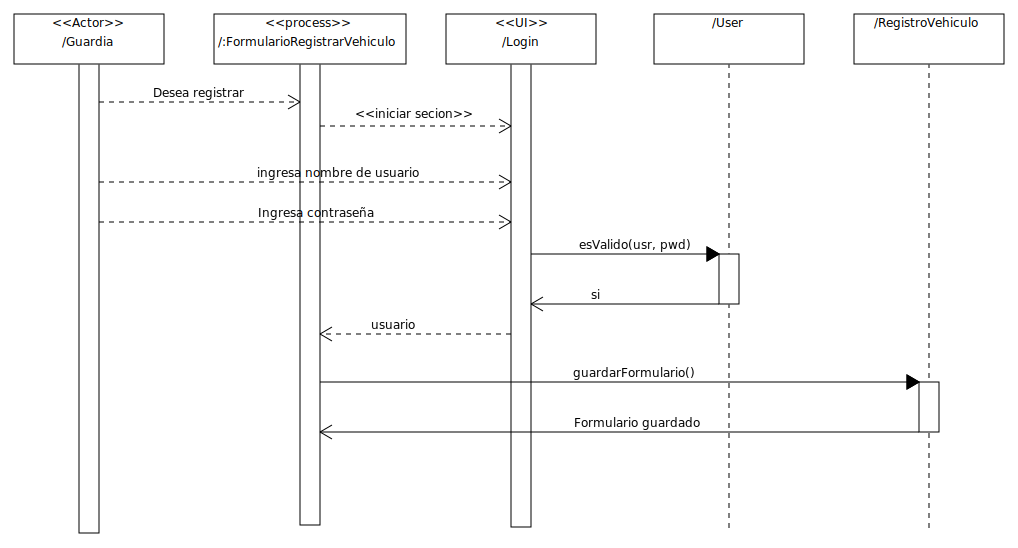
\includegraphics[width=1\textwidth]{figures/chapter4/SequenceDiagram21.svg}
    \caption[Diagrama de secuencia - Registro de vehículos]{
    Diagrama de secuencia para el Registro de vehículos}
  \end{center}
\end{figure}

\subsection{Registro de ingreso de personas}
Los guardias también tienen que estar atentos a toda {\it persona ajena} a la empresa
que quiere ingresar a las oficinas. Tiene que pedir un documento que lo identifique
y saber el motivo para lo que esta ingresando.

El archivo para este comportamiento sera {\it \bfseries ingresos.feature}

{\scriptsize
\begin{minted}{Gherkin}
Característica: Registro de personas
    Como un guardia
    Quiero registrar los ingresos y salidas de personas ajenas a la empresa
    Para tener un registro de ingresos

    Esquema del escenario: Registrar visita a oficinas
        Dado que ingresa una persona a las oficinas <oficina>
        Y con documento <documento>
        Y con numero de documento <num_doc>
        Y con el siguiente nombre <nombre>
        Y proviene de la ciudad <ciudad>
        Y con el siguiente motivo <motivo>
        Cuando registre a la persona
        Y el <num_doc> sea valido
        Entonces registro a la persona <nombre> con documento <num_doc> que ingreso a la oficina <oficina>

        Ejemplos:
            | oficina  | documento  | num_doc |   nombre     | ciudad |     motivo    |
            | muyurina | pasaporte  | 123456  | Marcelo Roca | br     | Reclamos ADSL |
            | central  | CI         | 654321  | Pedro Quispe | lpz    | Interac TV    |
\end{minted}
}

Para el registro de personas seguiría la siguiente secuencia.

\begin{figure}[h]
  \begin{center}
    \def\svgwidth{\columnwidth}
    \input{figures/chapter4/sequence_register_person.pdf_tex}
%    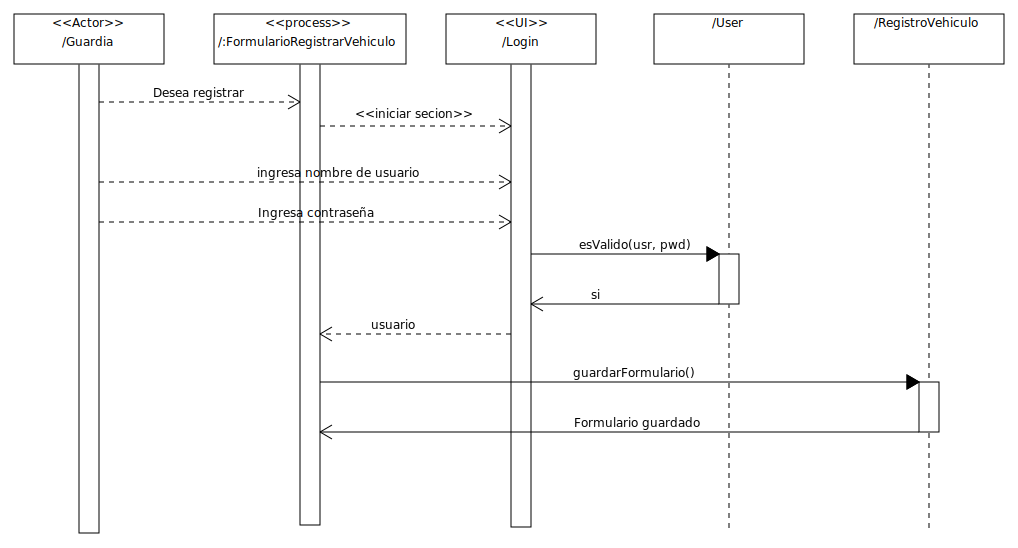
\includegraphics[width=1\textwidth]{figures/chapter4/SequenceDiagram21.svg}
    \caption[Diagrama de secuencia - Registro de personas]{
    Diagrama de secuencia para el Registro de Personas}
  \end{center}
\end{figure}

\subsection{Registro de mantenimiento}
Los vehículos siempre están en constante {\it mantenimiento},
pero también se vio la necesidad de tener un registro de que vehículos van al
taller para su mantenimiento y también programar mantenimientos preventivos.
Esta tarea la realiza el {\it Encargado de Vigilancia}.

El archivo para este comportamiento sera {\it \bfseries taller.feature}

{\scriptsize
\begin{minted}{Gherkin}
Característica: Registro de mantenimiento a vehículos
    Como un Encargado de Vigilancia
    Quiero registrar mantenimientos preventivos a los vehículos
    Para prevenir accidentes

    Esquema del escenario: Registrar o programar mantenimientos a vehículos
        Dado que el vehículo <interno> del parqueo <parqueo>
        Y su ultimo mantenimiento fue en fecha <fecha>
        Y con un kilometraje de <km_antiguo>
        Y con el siguiente motivo <motivo>
        Y su kilometraje actual es <km_actual>
        Y requiere el siguiente mantenimiento <mantenimiento>
        Cuando registre a el mantenimiento
        Y los datos de registro sean validos
        Entonces registro al vehículo <interno> del parqueo <parqueo> para mantenimiento

        Ejemplos:
            | parqueo  | interno | fecha       | km_antiguo | motivo           | km_actual | mantenimiento     |
            | muyurina | 167     | 12/01/2014  | 167944     | cambio de aceite | 187983    | cambio de aceite   |
            | sucre    | 54      | 25/04/2014  | 110456     | chequeo de motor | 150876    | revisión de motor |
\end{minted}
}

El diagrama de secuencia seria el siguiente:

\begin{figure}[h]
  \begin{center}
    \def\svgscale{0.6}
    \input{figures/chapter4/sequence_register_maintenance.pdf_tex}
%    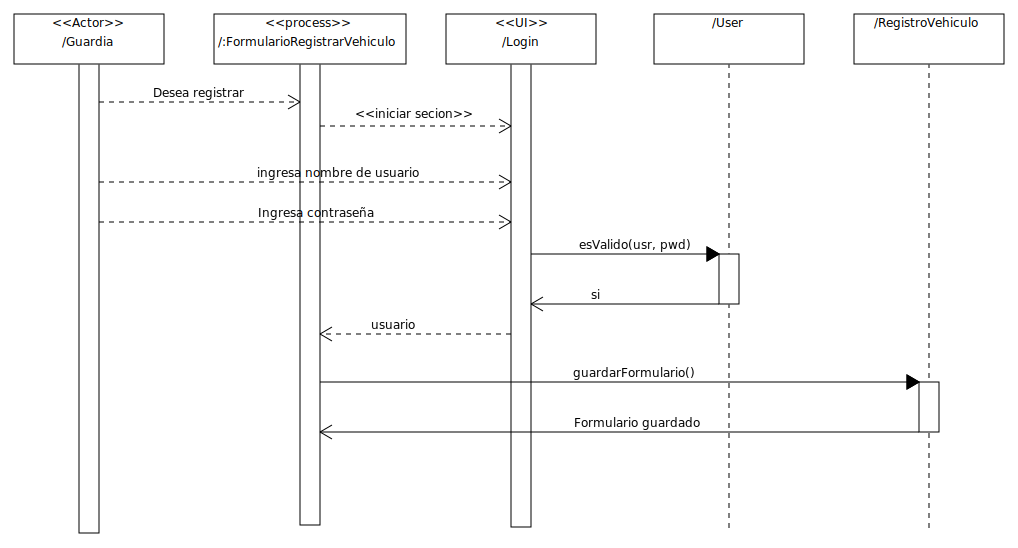
\includegraphics[width=1\textwidth]{figures/chapter4/SequenceDiagram21.svg}
    \caption[Diagrama de secuencia - Programar mantenimiento]{
    Diagrama de secuencia para programar mantenimiento}
  \end{center}
\end{figure}
\subsection{Reportes}
Los {\it reportes} es algo fundamental en el Sistema Web que se desarrolló, porque ayuda
a hacer los diferentes seguimientos de cada parqueo de los vehículos de la empresa.
Esta es una tarea que solo lo puede hacer el {\it Encargado de Vigilancia}.

El archivo para este comportamiento sera {\it \bfseries reportes.feature}

{\scriptsize
\begin{minted}{Gherkin}
Característica: Pagina de reportes
    Como un Encargado de Vigilancia
    Quiero sacar reportes de vehículos
    Para control interno

    Esquema del escenario: Sacar reportes de parqueos de un día
        Dado que necesito el reporte del parqueo <parqueo>
        Y solo de la fecha <fecha>
        Y lo quiero en formato <formato>
        Cuando ingreso los datos
        Entonces saco el reporte

        Ejemplos:
            | parqueo  | fecha       | formato |
            | muyurina | 10/06/2014  | pdf     |
            | sucre    | 15/07/2014  | excel   |

    Esquema del escenario: Sacar reportes de parqueos de un rango de fechas
        Dado que necesito el reporte del parqueo <parqueo>
        Y con fecha inicial <fecha_inicial>
        Y con fecha final <fecha_final>
        Y lo quiero en formato <formato>
        Cuando ingreso los datos
        Entonces saco el reporte

        Ejemplos:
            | parqueo  | fecha_inicial | fecha_final | formato |
            | muyurina | 10/03/2014    | 26/06/2014  | pdf     |
            | sucre    | 15/07/2014    | 26/06/2014  | excel   |
\end{minted}
}

La gran ventaja que tiene hacer estos escenarios en un lenguaje que entiende el
cliente es que puede dar su opinión de acuerdo a que variables quiere que también
se contemplen. Por ejemplo, en los anteriores escenarios para los reportes el
cliente vio la necesidad de tener también reportes que filtren por ítem de conductor
y por el número interno del vehículo. Dado estas aclaraciones con el cliente
el escenario quedaría de la siguiente manera:

{\scriptsize
\begin{minted}{Gherkin}
Esquema del escenario: Sacar reportes de parqueos
    Dado que necesito el reporte del parqueo <parqueo>
    Y con fecha inicial <fecha_inicial>
    Y con fecha final <fecha_final>
    Y con conductor <item_conductor>
    Y del vehículo <interno>
    Y lo quiero en formato <formato>
    Cuando ingreso los datos
    Entonces saco el reporte

    Ejemplos:
        | parqueo  | fecha_inicial | fecha_final | item_conductor | interno | formato |
        | muyurina | 10/03/2014    | 26/06/2014  | 505            | 167     | pdf     |
        | sucre    | 15/07/2014    | 26/06/2014  | 543            | I-02    | excel   |
\end{minted}
}

\begin{figure}[h]
  \begin{center}
    \def\svgwidth{\columnwidth}
    \input{figures/chapter4/sequence_report.pdf_tex}
%    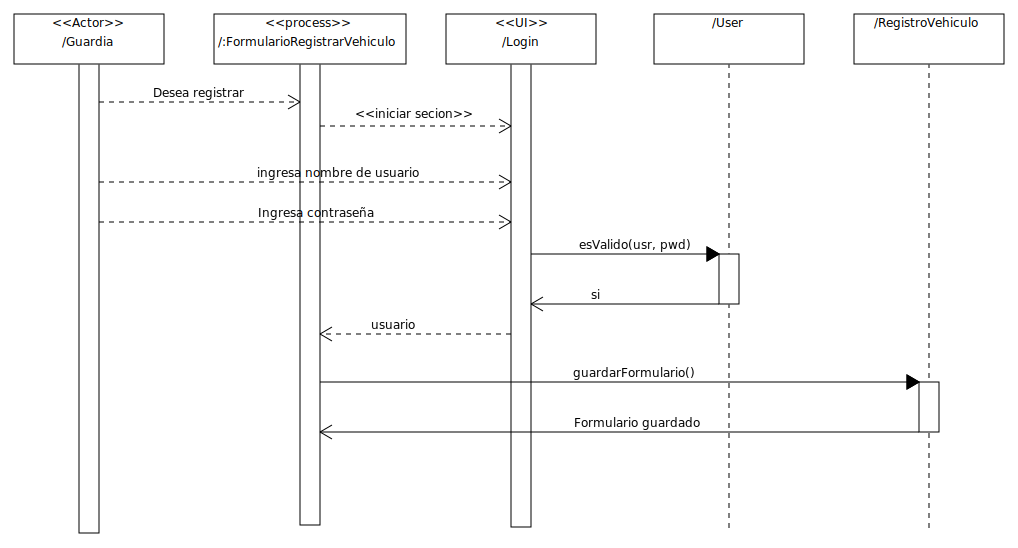
\includegraphics[width=1\textwidth]{figures/chapter4/SequenceDiagram21.svg}
    \caption[Diagrama de secuencia - Solicitud de reportes]{
    Diagrama de secuencia para la emisión de reportes}
  \end{center}
\end{figure}

\subsection{Notificaciones}
Las {\it notificaciones} ayuda al {\it Encargado de Vigilancia} a tomar ciertas medidas
de seguridad en la empresa, mas que todo respecto a los vehículos de la empresa y
los conductores.

Las notificaciones que se manejan están medidos por {\it bajo, medio y alto} solo
para estas alertas:

\begin{itemize}
  \item Un vehículo se queda en un parqueo diferente al que esta asignado - {\it medio}
  \item Un vehículo no llega a ningún parqueo - {\it alto}
  \item La licencia de conducir de un conductor ya esta por vencer - {\it alto}
\end{itemize}

El archivo para este comportamiento sera {\it \bfseries notificaciones.feature}

{\scriptsize
\begin{minted}{Gherkin}
Característica: Personalizar notificaciones
    Como un Encargado de Vigilancia
    Quiero dar valor a las notificaciones
    Para tomar medidas de seguridad

    Esquema del escenario: Cargar notificaciones
        Dado que manejo varias notificaciones
        Y con valores diferentes
        Cuando asigno valor a las notificaciones
        Entonces el sistema debe mandar alertas al encargado
\end{minted}
}

El diagrama de secuencia seria el siguiente:

\begin{figure}[h]
  \begin{center}
    \def\svgwidth{\columnwidth}
    \input{figures/chapter4/sequence_notifications.pdf_tex}
    \caption[Diagrama de secuencia - Administrar notificaciones]{
    Diagrama de secuencia para la administración de notificaciones}
  \end{center}
\end{figure}

Hasta este punto tenemos claro que es lo que tiene que hacer el sistema, que funcionalidades
debe cumplir, lo que veremos a continuación es como podemos darle un valor agregado
a todo los escenarios que escribimos con la ayuda de {\it Behave}

\section{Código generado para los test}
{\it Behave} es un interprete de Gherkin que lee todas las especificaciones que
escribimos y la forma de ejecutarlo es de la siguiente manera\footnote{En el Anexo A
se mostrará como instalar y configurar las diferentes herramientas}:

\vspace{0.5cm}
\texttt{\$ {\bfseries behave} \emph{registro.feature}}
\vspace{0.5cm}

\begin{figure}[h]
  \begin{center}
  \includegraphics[width=0.8\textwidth]{figures/chapter4/behave01m.png}
  \caption[Behave - primera ejecución]{Ejecución de behave}
\end{center}
\end{figure}

Todas las letras que nos muestra en color naranja son \emph{pasos} o \emph{steps}
sin definir y lo que nos muestra es un ejemplo de como podemos escribir estos
pasos. En el Anexo B de los \emph{Test de Ejecución} encontrará este código.

Los archivos \emph{.feature} tienen que estar en un directorio llamado {\bfseries
features} y el código escrito en python tiene que estar en otro directorio
llamado {\bfseries steps}, como puede ver a continuación.

\begin{figure}[h]
  \begin{center}
  \includegraphics[width=0.9\textwidth]{figures/chapter4/features_dir.png}
  \caption[Directorio features]{Organización del directorio \emph{features}}
\end{center}
\end{figure}

Esta es la forma correcta de organizar los features y los steps para Behave,
ademas en este directorio encontramos dos archivos nuevos que son:

\vspace{0.5cm}
\begin{mdframed}
\noindent
\texttt{
behave.ini \\
environment.py
}
\end{mdframed}
\vspace{0.5cm}

En {\bfseries behave.ini} escribimos variables de entorno que usara Behave al
momento de interpretar los archivos {\it .features}

\begin{verbatim}
[behave]
lang = es
\end{verbatim}

En este caso solo definimos el lenguaje en el que están escritos los escenarios.

En {\bfseries environment.py} inicializamos variables que usaremos al momento de
ejecutar los test.

\begin{verbatim}
import logging

def before_all(context):
    context.register_car = None
    context.parqueo_out = None
    context.km_out = None
    context.escaleras_out = None
    context.item_out = None
    context.date_out = None
    context.time_out = None
    context.dict_cars = {}
    context.warning = False

    if not context.config.log_capture:
        logging.basicConfig(level=logging.DEBUG)
\end{verbatim}

En los test que ejecutamos para este proyecto necesitamos que estén inicializadas
todas estas variables antes de todo.

Veamos como ejemplo la ejecución del {\it{\bfseries registro.feature}}:

\texttt{\$ {\bfseries behave} \emph{registro.feature}}

\begin{figure}[h]
  \begin{center}
  \includegraphics[width=1.1\textwidth]{figures/chapter4/behave_registro.png}
  \caption[Ejecución con Behave con error]{Ejecución con Behave escenario con error}
\end{center}
\end{figure}

En esta parte de la ejecución los colores nos interesan:

\begin{itemize}
  \item Verde. Se ejecuta el paso o {\it step} sin errores.
    \item Rojo. Ocurrió un error al ejecutar el paso.
    \item Azul. Pasos que no se ejecutaron.
    \item Naranja. Pasos no definidos.
\end{itemize}

En el escenario anterior hay un error, pero mas que un error es una alerta o futura
notificación en el sistema, ya que el vehículo ingresa al parqueo pero la persona
que ingresa con el vehículo no es la misma que lo saco. El sistema debe ser capaz
de agarrar esa alerta al momento de registrar y crear una notificación para el
encargado de Vigilancia.

En el siguiente escenario se ejecuta cada paso sin error:

\begin{figure}[h]
  \begin{center}
  \includegraphics[width=1.1\textwidth]{figures/chapter4/behave_registro02.png}
  \caption[Ejecución con Behave sin error]{Ejecución con Behave, escenario sin error}
\end{center}
\end{figure}

En esta fase inicial del desarrollo del producto tenemos claro de todas las
funcionalidades que espera ver el cliente en el sistema. Con todo lo desarrollado
hasta el momento y los test escritos en {\it Behave} se tiene como un primer
producto entregable, donde mostramos al cliente como pasan los test de acuerdo a
las especificaciones.

A continuación veremos como se hizo el modelo de la Base de Datos teniendo en
mente todo lo que hicimos hasta este punto. Hablando en términos de BDD hasta este
punto del desarrollo es trabajo de los testers y desarrolladores, de aquí para
adelante es solo trabajo de los desarrolladores.

\section{Modelo del sistema}
Según la definición original de BDD expuesta por Dan North\footnote{Dan North,
  principal impulsor en el desarrollo de BDD, \url{http://dantnorth.net}
consultado el 7/07/2014} nos dice:
\vspace{0.5cm}
\begin{mdframed}
{\it BDD is a second-generation, outside–in, pull-based, multiple-stakeholder,
  multiple-scale,  high-automation, agile methodology. It describes a cycle of
  interactions with well-defined outputs, resulting in the delivery of working,
  tested software that matters.
}
\end{mdframed}
\vspace{0.5cm}
BDD es pensar de afuera hacia adentro({\it outside-in}), es decir, una vez que
ya tenemos bien pensadas y trabajadas las funcionalidades, eso nos ayuda a tener una
idea más clara de lo que tenemos que hacer, como ser los modelos a implementar y
los roles que son necesarios crear.

\subsection{ACL - Lista de Control de Acceso}
Según las características podemos identificar dos roles: {\it Encargado de Vigilancia}
y {\it Guardia}, que son los que trabajaran con el sistema. Con ACL podemos definir
que puede y que no puede hacer cada rol, como vemos a continuación.

\vspace{1.0cm}

\begin{figure}[h]
  \begin{center}
  \includegraphics[width=0.7\textwidth]{figures/chapter4/acl.png}
  \caption[ACL - Roles del sistema]{ACL - Lista de Control de Acceso}
\end{center}
\end{figure}

\vspace{0.5cm}

En la figura anterior se muestra en las columnas las acciones sobre
un recurso y en las filas se tiene a los roles definidos en el sistema, en cada
intersección existe un valor de {\it falso} o {\it verdadero} que indica si el
rol tiene permiso de realizar esta acción o si no la tiene.

Esto es de acuerdo a las acciones que realizaran en el sistema:

\begin{itemize}
  \item como {\it guardia} debe ser capaz de registrar a los vehículos, es decir
    crear nuevos registros.
  \item como {\it guardia} debe ser capaz de ver todos los registros guardados.
  \item como {\it guardia} debe ser capaz de ver los reportes.
  \item como {\it encargado de vigilancia} debe ser capaz de editar registros.
  \item como {\it encargado de vigilancia} debe ser capaz de borrar registros.
  \item como {\it encargado de vigilancia} debe ser capaz de crear usuarios.
\end{itemize}

Este enfoque fue el más flexible que se encontró y es el que se implemento en la
aplicación.

Guiándonos por los escenarios que vimos en la sección 4.1 nosotros podemos ir
modelando con una idea mas clara de que actores o entidades necesitaremos para
cada característica.

\subsection{Registro de vehículos}
En base a nuestra primera característica que es el registro de vehículos y los
escenarios que la componen tendremos las siguientes entidades para un modelo ER.

%\begin{figure}[h]
%  \begin{center}
%    \def\svgwidth{\columnwidth}
%    \input{figures/chapter4/sequence_reg_car.pdf_tex}
%%    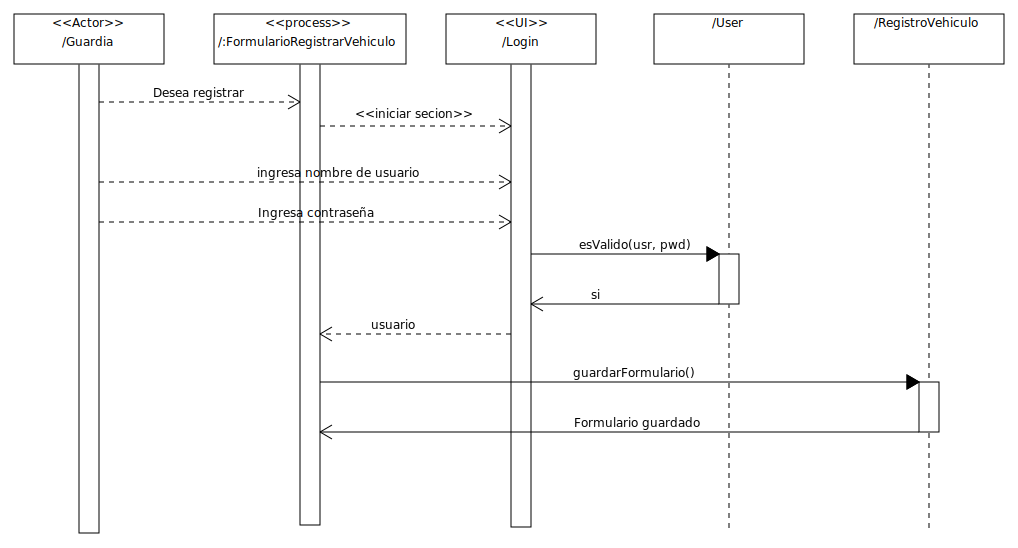
\includegraphics[width=1\textwidth]{figures/chapter4/SequenceDiagram21.svg}
%    \caption[Diagrama de casos de uso - Registro de vehículos]{
%    Diagrama de casos de uso para el Registro de vehículos}
%  \end{center}
%\end{figure}

\begin{itemize}
    \item User. Representa al usuario que usa el sistema, para este escenario el
      usuario es directamente el {\it guardia}.
    \item Employee. Es el empleado o funcionario que sale o retorna con el vehículo.
    \item BranchOffice. La sucursal de donde sale o ingresa el vehículo.
    \item Car. El Vehículo que es registrado.
    \item CarRegistration. La tabla donde se registra todos las salidas y retornos
        de los vehículos.
\end{itemize}

\begin{figure}[h]
  \begin{center}
    \includegraphics[width=0.6\textwidth]{figures/chapter4/er_registro.png}
    \caption[Modelo ER - Registro de vehículos]{Modelo ER para el registro de vehículos}
  \end{center}
\end{figure}

\newpage
\subsection{Registrar ingresos a oficinas}
En base al escenario de {\it ingreso de personas a la empresa} tenemos las
siguientes entidades con su modelo ER respectivo:

\begin{itemize}
    \item User. Representa al usuario que usa el sistema, para este escenario el
      usuario es directamente el {\it guardia}.
    \item Guest. Es la persona que esta ingresando a la empresa.
    \item RegisterGuest. La tabla donde se registran todos los ingresos.
\end{itemize}

\begin{figure}[h]
  \begin{center}
    \includegraphics[width=0.5\textwidth]{figures/chapter4/er_reg_visitas.png}
    \caption[Modelo ER - Registro de visitas]{Modelo ER para el registro de visitas}
  \end{center}
\end{figure}

\subsection{Programar mantenimiento}
Para programar mantenimiento de los vehículos se requieren las siguientes
entidades:

\begin{itemize}
    \item Car. El vehículo que es registrado.
    \item BranchOffice. La sucursal a la que pertenece el vehículo.
    \item MaintenanceProgram. La tabla donde se registra el mantenimiento programado.
\end{itemize}

\begin{figure}[h]
  \begin{center}
    \includegraphics[width=0.6\textwidth]{figures/chapter4/er_prog_mant.png}
    \caption[Modelo ER - Programar mantenimiento]{Modelo ER para programar mantenimiento}
  \end{center}
\end{figure}

\subsection{Registrar salida a taller}
Las entidades que están involucradas son las mismas que las de registro de ingreso
y salida de vehículos excepto que en este escenario tenemos una entidad más, que
es la entidad {\it MaintenanceWorkshop} o taller que es donde se registra cada
ingreso de un vehículo al taller de la empresa para su reparación o mantenimiento.

\begin{itemize}
    \item User. Representa al usuario que usa el sistema, para este escenario el
      usuario es directamente el {\it guardia}.
    \item Employee. Es el empleado o funcionario que sale o retorna con el vehículo.
    \item BranchOffice. La sucursal de donde sale o ingresa el vehículo.
    \item Car. El Vehículo que es registrado.
    \item CarRegistration. La tabla donde se registra todos las salidas y retornos
        de los vehículos.
    \item MaintenanceWorkshop. Tabla donde se registra el ingreso de los vehículos al
      taller de la empresa para su mantenimiento o reparación.
\end{itemize}

\begin{figure}[h]
  \begin{center}
    \includegraphics[width=0.8\textwidth]{figures/chapter4/er_salida_taller.png}
    \caption[Modelo ER - Registro de salida a taller]{Modelo ER para el registro de salida a taller}
  \end{center}
\end{figure}

\subsection{Administrar notificaciones}
Las notificaciones tienen la lógica de quien envía {\it sender} o la crea y para
quien es la notificación {\it owner}.

\begin{itemize}
    \item User. El usuario que envía la notificación o al que le corresponde.
    \item Notifications. Las notificaciones con sus respectivos dueños y con la
      prioridad que le corresponde.
    \item Notification. Las notificaciones creadas.
\end{itemize}

\begin{figure}[h]
  \begin{center}
    \includegraphics[width=0.8\textwidth]{figures/chapter4/er_notificaciones.png}
    \caption[Modelo ER - Notificaciones]{Modelo ER para el manejo de notificaciones}
  \end{center}
\end{figure}

\newpage
Aqui terminamos este desarrollo inicial del sistema, con los siguientes logros:

\begin{itemize}
    \item Funcionalidades escritas con BDD y probadas con Behave, mostrando así
      como se ejecuta cada funcionalidad.
    \item Modelo ER de la Base de Datos
\end{itemize}

En el siguiente capítulo veremos la parte del desarrollo web y el uso del
framework Django.

%En esta fase inicial del desarrollo del producto tenemos claro de todas las
%funcionalidades que espera ver el cliente en el sistema. Con todo lo desarrollado
%hasta el momento y los test escritos en {\it behave} se tiene como un primer
%producto entregable, donde mostramos al cliente como pasan los test de acuerdo a
%las especificaciones.

%En el libro \cite{Eigen1971} y en el libro \bibentry{Knuth1968} y usando el libro
%de latex \cite{goossens93}



%\renewcommand{\familydefault}{\sfdefault}
%\normalfont
%\setmonofont[Scale=MatchLowercase]{Consolas}
%\setmainfont{Times New Roman}

\begin{savequote}[75mm]
%Nulla facilisi. In vel sem. Morbi id urna in diam dignissim feugiat. Proin molestie tortor eu velit. Aliquam erat volutpat. Nullam ultrices, diam tempus vulputate egestas, eros pede varius leo.
%\qauthor{Quoteauthor Lastname}
\end{savequote}

%\chapter{Tecnologías de Desarrollo}
\chapter{Implementación del Sistema Web}

\newthought{Para} la implementación del sistema web se eligió trabajar con el
framework Django\footnote{Django \citeauthor{website:djangoproject}, \url{http://djangoproject.com}, consultado en
Julio de 2014}.

Django fue desarrollado en un ambiente ágil de redacción y se diseñó para que
las tareas comunes de desarrollo web fueran rápidas y simples. Esta escrito en
python y usa el paradigma conocido como Model Template View - MTV

%\section{Framework Django}

\subsection{Model Template View - MTV}
%Es interesante explicar que Django actualmente usa el patron MTV en lugar de MVC
%(Modelo Vista Controlador) pero basicamente es una forma diferente de llamar a los
%componentes del patron MVC. En Django el {\it controlador} se llama {\it view} y
%las {\it vistas} se las llama {\it template} o plantilla.

En la interpretación que hace Django al patrón MVC, el {\it view.py} describe los
datos que se presentan al usuario. Esto no es necesariamente como se ven los datos.
La {\it vista} indica qué datos puede ver el usuario no como los ve. Es una distinción
sutil.

Así, para Django una {\it ``View''} es la función de devolución en python para
una particular URL que esta definida en {\it urls.py}, debido a que la función
de devolución describe que datos son presentados.

Por otra parte Django hace un separacion del contenido de la presentacion que es
donde los {\it templates} o plantillas entran. En Django una ``vista'' describe
que datos son presentados, pero una vista normalmente delega a un {\it template},
el cual describe como los datos son presentados.

La figura a continuación muestra como interactuan el Modelo con la Vista y Template.

\begin{figure}[h]
  \begin{center}
    \includegraphics[width=0.4\textwidth]{figures/chapter5/Django_mvc.png}
    \caption[Model Template View - MTV]{Model View Template, Fuente: \url{http://djangoproject.org}}
  \end{center}
\end{figure}

Ahora llegamos a la pregunta ¿dónde viene a encajar el {\it ``controlador''}? En el caso
de Django, es probable que sea el Framework en si. La maquina que envía una
solicitud a la vista apropiada, de acuerdo con la configuración de los URL de Django
y las que definimos en nuestro proyecto que se encuentran en ``{\it urls.py}''.

Para entender a detalle este flujo que sigue Django tenemos la siguiente figura.

\begin{figure}[h]
  \begin{center}
    \includegraphics[width=0.6\textwidth]{figures/chapter5/DjangoFlow.png}
    \caption[El flujo de Django]{Una vista general del flujo de Django, Fuente: \url{http://hitesh.in/2009/django-flow/}}
  \end{center}
\end{figure}

\newpage

\begin{enumerate}
    \item El usuario hace una solicitud de una pagina.
    \item La solicitud llega a un {\it Request Middlewares} el cual lo manipula o
      responde a la solicitud.
    \item El {\it URLConf} busca la vista relacionada usando los {\it urls.py}
    \item {\it View Middlewares} es llamado, que manipula o responde a la
      solicitud.
    \item La función {\it view} es invocada.
    \item La vista puede opcionalmente tener acceso a los datos a través de los
        modelos.
    \item Todas las interacciones de modelo-a-DB se hacen a través de un {\it manager}.
    \item Las vistas podrían usar un {\it context} especial si es necesario.
    \item El context se pasa al {\it template} para la presentación.
\end{enumerate}

\begin{itemize}
  \item[a] Los templates usan {\it Filters} y {\it Tags} para la salida de la presentación.
  \item[b] La salida devuelta a la vista.
  \item[c] {\it HTTPResponse} envía a {\it Response Middlerwares}.
  \item[d] Cada una de las respuestas de los {\it Middlewares} puede enriquecer
    la respuesta o devolver completamente una nueva respuesta.
  \item[e] La respuesta es enviada la navegador del usuario.
\end{itemize}

\section{Estructura del Proyecto}
Ya con una vista general de como funciona Django vamos a ver como se estructura
un proyecto en Django.

\begin{verbatim}
flosite
    |-- manage.py
    |-- flosite (carpeta principal)
    |   |-- __init__.py
    |   |-- settings.py (archivo de Configuración del proyecto)
    |   |-- urls.py (urls que direcciona a las urls de las apps)
    |   `-- wsgi.py
    `-- app_one
    |   |-- templates/ (templates para el uso de este app)
    |   |-- __init__.py
    |   |-- models.py
    |   |-- views.py
    |   `-- urls.py (url que direcciona a las views de esta app)
    `-- app_two
    |   |-- templates/
    |   |-- __init__.py
    |   |-- models.py
    |   |-- views.py
    |   `-- urls.py
    `-- templates (Templates para el uso general del proyecto)
    |   |-- base.html
    |   |-- index.html
    `-- staticfiles
        |-- css/
        `-- js/

\end{verbatim}

Nuestro proyecto {\it flosite} cuenta con ocho aplicaciones, como ser: {\it account,
branchoffice, core, guest, maintenance, notifications, register, staff}. Algo
que es importante mencionar es que desde la versión 1.4 de Django los templates
se manejan diferente, ya que se tiene una carpeta {\it templates} para el uso
general del proyecto y cada aplicación maneja su propia carpeta de {\it templates}.

\begin{figure}[h]
  \begin{center}
    \includegraphics[width=0.3\textwidth]{figures/chapter5/appsdjango2.png}
    \caption[Estructura de una aplicación de un proyecto Django]{Estructura de una aplicación de un proyecto Django}
  \end{center}
\end{figure}

El archivo {\it flosite/urls.py} es muy importante que este bien configurado, ya
que este se encarga de delegar las peticiones que se hacen a las aplicaciones
correspondientes

\begin{verbatim}
$ less flosite/urls.py
\end{verbatim}

\newpage

{\scriptsize
\begin{verbatim}
from django.conf.urls import patterns, include, url
from django.views.generic import TemplateView
from django.conf import settings
from django.conf.urls.static import static
from django.contrib.staticfiles.urls import staticfiles_urlpatterns

from django.contrib import admin
admin.autodiscover()

urlpatterns = patterns('',
    url(r'^$', TemplateView.as_view(template_name='index.html'), name="home"),
    url(r'^accounts/', include('userena.urls')),
    url(r'^messages/', include('userena.contrib.umessages.urls')),
    url(r'^staff/', include('staff.urls')),
    url(r'^branchoffice/', include('branchoffice.urls')),
    url(r'^notifications/', include('notifications.urls')),
    url(r'^maintenance/', include('maintenance.urls')),
    url(r'^guest/', include('guest.urls')),
    url(r'^register/', include('register.urls')),
    url(r'^admin/', include(admin.site.urls)),
) + static(settings.MEDIA_URL, document_root=settings.MEDIA_ROOT)

urlpatterns += staticfiles_urlpatterns()
\end{verbatim}
}

Gráficamente tendríamos lo siguiente:

\begin{figure}[h]
  \begin{center}
    \def\svgwidth{\columnwidth}
    \input{figures/chapter5/urls.pdf_tex}
    \caption[Django Urls]{flosite/urls.py}
  \end{center}
\end{figure}

\section{Configuración del proyecto}
La configuración del proyecto se encuentra en {\it flosite/settings.py}, no
mostraremos todo el archivo de configuración solo resaltaremos las partes más
importantes.

\subsection{El archivo settings.py}
Al crear un proyecto con Django\footnote{Vea el apéndice de Instalación para
más detalles} se crea un archivo settings.py donde uno tiene que modificar el
archivo con los datos correspondientes.

\begin{verbatim}
$ less flosite/settings.py
\end{verbatim}

\begin{verbatim}
DATABASES = {
    'default': {
         # Add 'postgresql_psycopg2', 'mysql', 'sqlite3' or 'oracle'.
        'ENGINE': 'django.db.backends.mysql',
        'NAME': 'nombre_base_de_datos',
        'USER': '#########',
        'PASSWORD': '############',
        'HOST': '',
        'PORT': '', # Set to empty string for default.
    }
}
\end{verbatim}

Para instalar las aplicaciones que hemos creado en el archivo {\it settings.py}
se tiene otra sección especifica para esto:

\begin{verbatim}
INSTALLED_APPS = (
    # default
    'django.contrib.auth',
    'django.contrib.contenttypes',
    'django.contrib.sessions',
    'django.contrib.sites',
    'django.contrib.messages',
    'django.contrib.staticfiles',

    # ....

    # project flosite
    'accounts',
    'staff',
    'guest',
    'branchoffice',
    'guest',
    'register',
    'core',
    'notifications',
    'maintenance',
\end{verbatim}

Todas las aplicaciones que se mencionan en esta sección son las que se instalan
al momento de hacer un {\it syncdb}.\footnote{Vea el apéndice de Instalación para
mas detalles}

\begin{verbatim}
$ python manage.py syncdb
\end{verbatim}

\section{Aplicaciones extras para el sistema}
Teniendo en cuenta las herramientas y bondades que ofrece Django, para el proyecto
usamos las siguientes aplicaciones ya desarrolladas.

\begin{verbatim}
INSTALLED_APPS = (
    # ....

    #extras
    'bootstrap_toolkit',
    'bootstrap3_datetime',
    'pagination',
    'debug_toolbar',
    'userena',

  # ....
)
\end{verbatim}

\begin{itemize}
    \item bootstrap\_toolkit: nos ofrece todo el diseño web y paginas de estilo
      necesarias.
    \item bootstrap3\_datetime: nos permite el manejo de calendarios en los forms.
    \item pagination: Esta herramienta es muy importante para la paginación de tablas.
    \item debug\_toolbar: Una herramienta útil para debug.
    \item userena: Para el manejo de usuarios y sus perfiles.
\end{itemize}

\begin{figure}[h]
  \begin{center}
    \includegraphics[width=0.6\textwidth]{figures/chapter5/homepage.png}
    \caption[Página de inicio del Sistema Web]{Página de inicio del Sistema Web}
  \end{center}
\end{figure}

\section{Formularios para los registros}
Para el sistema tenemos tres formularios: {\it Registro de vehículos, Registro
de Personas, Reportes}

\subsection{Registro de Vehículos}
Los formularios para los registro se encuentra en {\it register/forms.py}

\begin{verbatim}
$ less register/forms.py
\end{verbatim}

\begin{verbatim}
from django import forms

class RegisterKmForm(forms.Form):
    r_automotive = forms.CharField(widget=forms.TextInput(attrs={...}))
    r_km_revert = forms.BooleanField(required=False)
    r_date   = forms.DateField(widget=BootstrapDateInput(attrs={...}))
    r_hour   = forms.TimeField(widget=forms.TextInput(attrs={...}))
    r_km     = forms.IntegerField(label=_('output_km'), widget=...)
    r_driver = forms.CharField(widget=forms.TextInput(attrs={...}))
    r_ladder = forms.CharField(required=False)
    r_obs    = forms.CharField(widget=forms.Textarea, required=False)

    # validators
    def ...
\end{verbatim}
A estos formularios se los llama desde {\it register/views.py} y lo carga en el
template {\it register/templates/register\_form.html} para tener el siguiente
formulario:

El código de {\it views.py} para registro de vehículos seria el siguiente:

\begin{alltt}
from django.shortcuts import render, ...
from register.forms import \emph{RegisterKmForm}, ...

@login_required
@csrf_protect
@permission_required_or_403('register.add_register_automotive')
def form_car(request):
    ....
    if request.method == 'POST':
        form = \emph{RegisterKmForm(request.POST)} # Esta linea llama al form
        if form.is_valid():
            ....
    else:
      form = \emph{RegisterKmForm()}
    return render(request, 'register_form.html', {'form': form})
\end{alltt}

La ultima linea es la que se encarga principalmente de renderizar el template con
el formulario.

\begin{verbatim}
return render(request, 'register_form.html', {'form': form})
\end{verbatim}

Y con todo, tendríamos la siguiente vista:

\begin{figure}[h]
  \begin{center}
    \includegraphics[width=0.8\textwidth]{figures/chapter5/registro2.png}
    \caption[Formulario de Registro de Vehículos]{Formulario de Registro de Vehículo}
  \end{center}
\end{figure}

\newpage

\subsection{Registro de Personas}
El formulario para el registro de personas se encuentra también en {\it register/forms.py}
y seria el siguiente:

\begin{verbatim}
class RegisterPersonForm(forms.Form):
    LOCALE_CHOICES = (
        ('cba', 'Cochabamba'),
        ('lpz', 'La Paz'),
        ('scz', 'Santa Cruz'),
        ('pnd', 'Pando'),
        ('ben', 'Beni'),
        ('oru', 'Oruro'),
        ('pts', 'Potosi'),
        ('tja', 'Tarija'),
        ('scr', 'Chuquisaca'),
        ('---', _('none')),
        )

    GENDER_CHOICES = (
        ('H', 'Hombre'),
        ('M', 'Mujer')
    )
    identity_document = forms.CharField(required=True, widget=...)
    city = forms.CharField(required=True, widget=forms.Select(...))
    first_name = forms.CharField(required=True)
    last_name = forms.CharField(required=True)
    gender = forms.CharField(required=True, widget=forms.Select(...))
    reason = forms.CharField(required=True, widget=forms.Textarea)
\end{verbatim}

La llamada desde el {\it views.py}

\begin{alltt}

from register.forms import RegisterPersonForm

@login_required
@csrf_protect
@permission_required_or_403('register.add_register_person')
def form_register_person(request):
    if request.method == 'POST':
        form = \emph{RegisterPersonForm(request.POST)}
        if form.is_valid():
            ...
            return HttpResponseRedirect('/register/persons')
    else:
        form  = \emph{RegisterPersonForm()}
    return render(request, 'form_register_person.html', {'form': form})
\end{alltt}

Esta vista llama al template {\it form\_register\_person.html}

\begin{figure}[h]
  \begin{center}
    \includegraphics[width=0.8\textwidth]{figures/chapter5/registro_personas.png}
    \caption[Formulario de Registro de Personas]{Formulario para el Registro de Personas}
  \end{center}
\end{figure}

\newpage

\subsection{Reportes}
El formulario para los reportes se encuentra {\it report/forms.py}

\begin{verbatim}
class ReportForm(forms.Form):
    generate_pdf = forms.BooleanField(required=False)
    generate_excel = forms.BooleanField(required=False)
    parking = forms.ModelChoiceField(queryset=LocaleParking.objects.all(),
                                     empty_label="(seleccione un parqueo)")
    today = forms.DateField(label='today', widget=BootstrapDateInput(...))
    date_begin = forms.DateField(widget=BootstrapDateInput(...)
    date_end = forms.DateField(widget=BootstrapDateInput(format="%d/%m/%Y"), ..)
    internal_num_car = forms.CharField(max_length=10, required=False)
    item_driver = forms.CharField(max_length=10, required=False)
\end{verbatim}

La llamada desde el vista es la siguiente y se encuentra en {\it report/views.py}

\begin{alltt}
@login_required
def home(request):
    if 'csrfmiddlewaretoken' in request.GET:
        form = \emph{ReportForm(request.GET)}
        if form.is\_valid():
            .....
    else:
        return render\_to\_response('report/list.html', {'report': report.order\_by(...)})
    else:
        form = \emph{ReportForm()}

    return render(request, 'report/report.html', {'form': form})
\end{alltt}

Esta vista llama al template {\it report/report.html}

\begin{figure}[h]
  \begin{center}
    \includegraphics[width=0.8\textwidth]{figures/chapter5/reportes.png}
    \caption[Formulario para Reportes]{Formulario para Reportes}
  \end{center}
\end{figure}


\begin{savequote}[75mm]
%Nulla facilisi. In vel sem. Morbi id urna in diam dignissim feugiat. Proin molestie tortor eu velit. Aliquam erat volutpat. Nullam ultrices, diam tempus vulputate egestas, eros pede varius leo.
%\qauthor{Quoteauthor Lastname}
\end{savequote}

\chapter{Pruebas del Sistema}

\newthought{En} el capítulo tres vimos como la metodología BDD es una herramienta útil que
fomenta la colaboración entre desarrolladores, testers y clientes. Entendimos
como BDD es una técnica de desarrollo ágil de software.

En el capítulo cuatro vimos la aplicación de BDD en el proyecto e hicimos los
escenarios respectivos para cumplir los requerimientos de funcionalidad del
sistema.

\begin{itemize}
    \item Registro de Vehículos
    \item Registro de Ingreso de personas
    \item Registro de mantenimiento
    \item Reportes
    \item Notificaciones
\end{itemize}

En este capítulo mostraremos como esos escenarios que ya definimos nos sirven
para hacer las pruebas finales.

Los escenarios y el código que desarrollamos para que pasen los tests eran solo
una muestra de como el sistema iba a cumplir todos los requerimientos de
funcionalidad.

Hasta este punto del proyecto ya se tiene el sistema completo. Y ahora es cuando
usaremos esos mismos escenarios para mostrar como el sistema cumple con las
funcionalidades exigidas.

Para realizar estas pruebas necesitaremos de dos herramientas mas en el
entorno virtual de desarrollo.

\begin{itemize}
  \item django-behave\footnote{Django-Behave, desarrollado por \citeauthor*{website:djangobehave}}
  \item splinter\footnote{Splinter, desarrollado por \citeauthor{website:splinter}}
\end{itemize}

\section {django-behave}
Es un TestRunner de Django para el modulo de Behave BDD, ya en el capítulo tres
y cuatro vimos como trabaja {\it behave} con BDD.

\subsection{Instalación}
Para la instalación primero entraremos a nuestro entorno virtual de desarrollo y
usando {\it pip}\footnote{PIP, es un manejador de paquetes de Python} lo
instalaremos.
\begin{verbatim}
project$ source ~/env/bin/active
(env)project$ pip install django-behave
\end{verbatim}

\subsection{Configuración}
Una vez instalado django-behave pasamos a hacer la configuración en el archivo
{\it settings.py} y hacemos los cambios como se muestra a continuación.
\begin{verbatim}
INSTALLED_APPS = (
    ..
    'django_behave',
)

TEST_RUNNER = 'django_behave.runner.DjangoBehaveTestSuiteRunner'
\end{verbatim}

\section {splinter}
Splinter\footnote{Splinter, \url{http://splinter.cobrateam.info/en/latest/},
consultado en noviembre de 2014} es una herramienta Open Source para hacer
pruebas en aplicaciones web usando Python. Permite automatizar acciones dentro
del navegador, como visitar URLs e interactuar con los items.

\subsection{Instalación}
Para instalarlo usaremos {\it pip} como en los casos anteriores y siempre
trabajando dentro de nuestro entorno virtual:

\begin{verbatim}
(env)project$ pip install splinter
\end{verbatim}

Enhorabuena, ya tenemos instalado {\it django-behave} y {\it splinter}, ahora la
forma de usarlo es de la siguiente manera:

\begin{verbatim}
(env)project$ python manage.py test app
\end{verbatim}

Como ya tenemos configurado django-behave en {\it settings.py} el archivo
{\it manage.py} reconoce la orden {\it test} y lo que viene después es el
nombre de la aplicación que en el ejemplo solo se lo llama {\it app}.

Pero {\it splinter} no se ejecuta de manera mágica, necesitamos decirle a los
{\it features} de BDD de cada aplicación de nuestro proyecto que debe usar
splinter al momento de ejecutar los tests.

\section{Configuración de los escenarios}
En el capítulo cuatro pusimos todos los escenarios en una misma carpeta {\it features}
y cuando lo ejecutábamos con {\it behave} recorría todos los escenarios.

Pero ahora, como ya tenemos el sistema completo con sus aplicaciones respectivas
para cada funcionalidad vamos a llevar los escenarios a la aplicación que le
corresponde, veamos el caso de {\it accounts}.

\begin{verbatim}
flosite
    |-- manage.py
    |-- flosite (carpeta principal)
    |   `-- ...
    |-- accounts/
    |  |-- features
    |  |   |-- behave.ini
    |  |   |-- environment.py
    |  |   |-- login.feature
    |  |   `-- steps
    |  |       `-- step_login.py
    |  |-- __init__.py
    |  |-- models.py
    |  |-- urls.py
    |  `-- views.py
    |-- ...
\end{verbatim}

En la aplicación {\it accounts} ahora tenemos la carpeta {\it features} y es ahí
donde están los archivos de Configuración y su escenario {\it login.feature},
veamos {\it behave.ini}:

\begin{verbatim}
[behave]
lang = es
\end{verbatim}

En este archivo le decimos de manera explicita que los escenarios están escritos
en {\it Español}.

El archivo {\it environment.py} es el que mas nos interesa ahora, porque es ahí
donde le decimos a {\it django-behave} que use splinter al momento realizar los
tests.

\begin{verbatim}
from splinter.browser import Browser

def before_all(context):
    context.browser = Browser()

def after_all(context):
    context.browser.quit()
    context.browser = None
\end{verbatim}

El método {\it before\_all}, se encarga de que antes de cualquier cosa inicialice
el Browser o el navegador.

El método {\it after\_all}, se encarga de que después que realice todos los pasos
cierre el navegador.

\section{Escenario Account}
Como ya mencionamos, trabajaremos con {\it accounts} para ver como se ejecuta
el test con splinter paso a paso. Veamos el archivo {\it login.features}:

{\scriptsize
\begin{minted}{Gherkin}
# language: es

Característica: Pagina principal
    Como un guardia
    Quiero ingresar al sistema
    Para registrar ingresos

    Esquema del escenario: Iniciar sesión
        Dado que ingreso al sistema con el url "http://127.0.0.1:8000/"
        Y voy a la opcion "Ingresar"
        Y entro con mi nombre de usuario <username>
        Y mi contraseña <password>
        Cuando oprima el boton "Ingresa"
        Entonces ingreso al sistema y leo el mensaje "Bienvenido"

        Ejemplos:
            | username | password |
            | benjamin | asdf     |
\end{minted}
}

A diferencia de los escenarios que ya vimos, aquí le decimos que tiene que entrar
a una dirección URL.

Una vez hecho esto en la carpeta {\bfseries steps} escribimos el código necesario
para este escenario en el archivo {\it step\_login.py}.

\begin{verbatim}
# encoding: utf-8

from behave import given, when, then

@given(u'que ingreso al sistema con el url "{url}"')
def impl(context, url):
    br = context.browser
    br.visit(url)

@given(u'voy a la opcion "{option}"')
def impl(context, option):
    link = context.browser.find_link_by_text(option).first
    assert link
    link.click()

@given(u'entro con mi nombre de usuario {usr}')
def impl(context, usr):
    context.browser.fill('identification', usr)
    context.user = usr
    assert usr

@given(u'mi contraseña {pwd}')
def impl(context, pwd):
    context.browser.fill('password', pwd)
    context.password = pwd
    assert pwd

@when(u'oprima el boton "{btn}"')
def impl(context, btn):
    button = context.browser.find_by_value(btn).first
    assert button
    button.click()

@then(u'ingreso al sistema y leo el mensaje "{msg}"')
def impl(context, msg):
    assert msg in context.browser.html
\end{verbatim}

Cada método recibe como atributo a {\it context} y como en el archivo
{\it environment.py} ya lo inicializamos con splinter, solo tenemos que llamar
a sus métodos e ir recorriendo la pagina siguiendo los pasos escritos
en {\it login.features}.

Una vez escrito y configurado todo esto ejecutamos el test:

\begin{verbatim}
(env)project$ python manage.py test accounts
\end{verbatim}

Cuando se ejecuta el test llama a {\it splinter} que a la vez ejecuta un navegador
de pruebas donde recorre los pasos que hemos definido en los escenarios.

Esto podemos verlo en el siguiente vídeo que es de mi autoría puesto en youtube.com
con el siguiente título {\it BDD, django-behave and splinter}\footnote{BDD,
django-behave and splinter: publicado el 2 de diciembre de 2014} en la URL: \url{http://youtu.be/KT6DCFfCFnY}


\begin{savequote}[75mm]
%Nulla facilisi. In vel sem. Morbi id urna in diam dignissim feugiat. Proin molestie tortor eu velit. Aliquam erat volutpat. Nullam ultrices, diam tempus vulputate egestas, eros pede varius leo.
%\qauthor{Quoteauthor Lastname}
\end{savequote}

\chapter{Puesta en producción}

\newthought{Para} la puesta en producción del sistema es preciso tomar en cuenta
otras herramientas como el Sistema Operativo donde se ejecutara el sistema,
el Servidor Web que usaremos para desplegar el proyecto, etc.

\section{Servidor Debian Linux}
Debian es una distribución de Linux, un Sistema Operativo Libre con acceso en línea
a los diferentes repositorios que tiene.

Se eligió Debian por el soporte estable que tiene para servidores y por lo practicó
que es al momento de instalar los paquetes de software.

La versión que usaremos para el proyecto es Debian 7.7 que tiene el nombre de
{\it Wheezy}.

\section{Servidor Web Nginx}
Nginx es un Servidor Web ligero y Libre, ademas de eso es de alto rendimiento.
Es conocido por su estabilidad, gran conjunto de características, configuración
simple, y bajo consumo de recursos.
También cuenta con un buen soporte de para FastCGI. Nginx y FastCGI\footnote{FastCGI
es un protocolo para interconectar con un Servidor Web} es una buena elección
al momento de desarrollar con Django y es lo que usaremos para el proyecto,
aunque no es el único camino.

La forma de instalar en Debian es la siguiente:

\begin{verbatim}
# aptitude install nginx
\end{verbatim}

Y la versión que instalará y la que usaremos es la 1.2.1

\section{Base de datos MySQL}
MySQL es un sistema de Base de Datos estable, rápido, multi-usuario y multi-hilo.
La principal meta de MySQL es ser rápido, robusto y fácil de usar.

La forma de instalar es la siguiente:

\begin{verbatim}
# aptitude install mysql-server
\end{verbatim}

Esto nos instalará la versión 5.5 de MySQL.

\section{Instalación y Configuración del Sistema}
Para no tener conflictos de versiones de paquetes de software en el servidor
crearemos un entorno virtual para el proyecto donde ahí instalaremos todos los
paquetes que son requeridos para el funcionamiento del sistema.

Para ello necesitamos instalar en el servidor {\it virtualenv}, esto nos permitirá
crear el entorno virtual que necesitamos para el proyecto, pero antes debemos
instalar {\it python-pip} y una vez hecho esto con {\it pip} instalaremos
{\it virtualenv}.

\begin{verbatim}
# aptitude install python-pip
# pip install virtualenv
\end{verbatim}

\begin{itemize}
  \item {\it pip} - Es un manejador de paquetes de software para Python
  \item {\it virtualenv} - Es una herramienta para mantener las dependencias
    de las versiones de los paquetes de software requeridas por los diferentes
    proyectos y separarlas.
\end{itemize}

Ahora creamos nuestro entorno virtual llamado {\it env} y lo activamos. Y esto
lo hacemos como un usuario normal ya no como {\it root}.

\begin{verbatim}
user:~$ virtualenv env
user:~$ source env/bin/activate
(env)user:~$
\end{verbatim}

En Debian y en otras distribuciones Linux se tiene {\it /var/www/} para los sitios
Web y es ahí donde copiaremos el sistema {\it /var/www/flosite/}.

Pero antes de instalar el sistema crearemos la Base de Datos y un usuario con
privilegios.

\begin{verbatim}
mysql> create database projectdb;
mysql> create user userdb identified by 'xxxxxx';
mysql> grant all privileges on projectdb.* to userdb;
\end{verbatim}

Ingresamos a la carpeta del proyecto pero primero activamos el entorno virtual
que ya creamos anteriormente.

\begin{verbatim}
user:~$ source env/bin/activate
(env)user:~$ cd /var/www/flosite/
(env)user:/var/www/flosite$
\end{verbatim}

Para facilitar la instalación tenemos el siguiente archivo
{\it requirements/project.txt}, ahí se tiene todas las dependencias del proyecto
y lo usamos de la siguiente manera:

\begin{verbatim}
(env)user:/var/www/flosite$ pip install -r requirements/project.txt
\end{verbatim}

Hasta este punto ya tenemos todo lo necesario para que el sistema se ejecute sin
problemas, ahora vamos a sincronizar el proyecto con la Base de Datos para la
creación de las tablas.

Primero configuramos {\it settings.py} para la Base de Datos.

\begin{verbatim}
DATABASES = {
    'default': {
        'ENGINE': 'django.db.backends.mysql',
        'NAME': 'projectdb',
        'USER': 'userdb',
        'PASSWORD': 'xxxxxxx',
        'HOST': '',
        'PORT': '',
    }
}
\end{verbatim}

Una vez editado y guardado {\it settings.py} sincronizamos el proyecto con la
Base de Datos y usamos la instrucción {\it syncdb} para ello.

\begin{verbatim}
(env)user:/var/www/flosite$ python manage.py syncdb
\end{verbatim}

Y para terminar levantamos el sistema:

\begin{verbatim}
(env)user:/var/www/flosite$ python manage.py runserver
\end{verbatim}

En el navegador del servidor ingresamos al URL \url{http://127.0.0.1:8000} y
efectivamente el sistema esta ejecutándose, pero no pueden ingresar desde otras
maquinas, como ya contamos con una IP pública hacemos lo siguiente:

\begin{verbatim}
(env)user:/var/www/flosite$ python manage.py runserver 0.0.0.0:8000
\end{verbatim}

Ahora todos pueden ingresar al sistema usando el IP del servidor como URL
\url{http://xxx.xxx.xxx.xxx:8000}

Pero ejecutar el sistema de esta forma es incomodo y ademas que tenemos que
ejecutarlo manualmente. En la siguiente sección veremos como automatizar esta
tarea en el servidor.

\section{Configuración en el servidor}
Bien, ahora es el turno de Nginx y Debian para el paso final de la puesta en
producción del sistema.

\subsection{Nginx}
Vamos a los archivos de configuración de Nginx en {\it /etc/nginx/} y en
{\it sites-available} creamos el archivo {\it flosite.conf}

\begin{verbatim}
root:~# cd /etc/nginx/sites-available/
root:/etc/nginx/sites-available# touch flosite.conf
\end{verbatim}

En {\it flosite.conf} copiamos las siguientes lineas.

\begin{verbatim}
server {
    listen 80;
    server_name IP.de.nuestro.servidor;
    access_log /var/log/nginx/flosite.access.log;
    error_log /var/log/nginx/flosite.error.log;

    location /static/ { # STATIC_URL
        alias /var/www/flosite/staticfiles/; # STATIC_ROOT
        expires 30d;
    }

    location /static/admin/ { # STATIC_ADMIN
        alias /home/user/env/lib/python2.7/site-packages/django/..../admin/;
        expires 30d;
    }

    location /media/ { # MEDIA_URL
        alias /var/www/flosite/media/; # MEDIA_ROOT
        expires 30d;
    }

    location / {
        include fastcgi_params;
        fastcgi_pass 0.0.0.0:8080;
        fastcgi_split_path_info ^()(.*)$;
        fastcgi_read_timeout    20m;
    }
}
\end{verbatim}

Ahora creamos un enlace simbólico en la carpeta {\it sites-enabled}

\begin{verbatim}
root:/etc/nginx# ln -s sites-available/flosite.conf sites-enabled/
\end{verbatim}

Reiniciamos Nginx para que reconozca la nueva configuración que hemos cargado.

\begin{verbatim}
# service nginx restart
\end{verbatim}

Pero aun nos falta algo, si se fijo en la sección de {\it location} necesitamos
pasarle un fastcgi a nuestra configuración de Nginx, para esto ejecutamos el
siguiente comando:

\begin{verbatim}
(env)user:/var/www/flosite$ python manage.py runfcgi host=0.0.0.0 port=8080
(env)user:/var/www/flosite$
\end{verbatim}

Esto crea el {\it fastcgi} que necesita la configuración que creamos en Nginx.

Si vamos al navegador e ingresamos con nuestra IP, efectivamente esta funcionando
\url{http://ip.de.nuestro.servidor/}

Pero aun hay un comando que hay que escribir manualmente. Ahora es el turno de
Debian Linux.

\subsection{Configuración en el Servidor Debian Linux}
Para automatizar la tarea de levantar el sistema al momento de iniciar el servidor
necesitamos usar {\it update-rc.d} que es el comando usado para decidir la secuencia
y el runlevel de ejecución del script que crearemos.

Creamos nuestro script {\it flosite} en {\it /etc/init.d/}

\begin{verbatim}
# touch /etc/init.d/flosite
\end{verbatim}

Ahora copiamos las lineas a continuación en el archivo creado.

\begin{verbatim}
#! /bin/bash
#
### BEGIN INIT INFO
# Provides:          flosite
# Required-Start:    mysql
# Required-Stop:     mysql
# Default-Start:     2 3 4 5
# Default-Stop:      0 1 6
# Short-Description: Inicia el sistema de flosite
# Description:       Este script fue escrito por Benjamin Perez
### END INIT INFO

# Este script es para levantar el sistema de seguridad industrial
echo "This part always gets executed"

case "$1" in
  start)
    echo "Starting flosite"
    echo "Please waith ....."
    source /home/user/env/bin/activate
    cd /var/www/flosite
    python manage.py runfcgi host=0.0.0.0 port=8080
    deactivate
    echo "Done" 
    ;;
  stop)
    echo "Stopping flosite"
    echo "Please waith ..."
    # TODO
    echo "Done"
    ;;
  restart)
    echo "Restarting flosite"
    echo "Please waith ....."
    # TODO
    ;;
  *)
    echo "Usage: /etc/init.d/flobasic {start|stop|restart}"
    exit 1
    ;;
esac

exit 0

\end{verbatim}

En este script algo que es muy importante son estas lineas:

\begin{verbatim}
# Required-Start:    mysql
# Required-Stop:     mysql
\end{verbatim}

Con estas lineas le decimos que nuestro script se ejecute o se detenga una vez
que ya inicio o se detuvo MySQL. Esto es importante por que si el script se
ejecuta antes de MySQL nos dará error y no podremos ingresar al sistema.

Ahora le damos permisos de ejecución:

\begin{verbatim}
# chmod +x /etc/init.d/flosite
\end{verbatim}

Finalmente ejecutamos {\it update-rc.d} para que el script se ejecute automáticamente
al iniciar el servidor.

\begin{verbatim}
# update-rc.d /etc/init.d/flosite defaults
\end{verbatim}

Al usar la opción {\it defaults} update-rc.d creará enlaces para iniciar el servicio
en los runlevels 2345 y detendrá el servicio en los runlevels 016.

Los {\it runlevels} básicamente se refieren a los diferentes niveles que tiene
un Servidor Linux para iniciar y parar servicios.

Con esto ya tenemos un servidor listo para ejecutar automáticamente el proyecto.


\begin{savequote}[75mm]
% Algun mensaje
%\qauthor{Algun Autor}
\end{savequote}

\chapter{Conclusiones y recomendaciones}

\section{Conclusiones}
El sistema se pudo terminar satisfactoriamente.Se logro alcanzar las expectativas
que se pusieron desde un inicio, cumpliendo todas las funcionalidades que se
necesitan para el control de los vehículos como de las personas que ingresan a
las diferentes oficinas.

Algunas conclusiones puntuales:

\begin{itemize}
  \item El uso de una metodología ágil como es BDD, fue excelente al
    momento de entender las funcionalidades exigidas por el usuario final.

  \item El uso de Django que es un Framework Web de alto nivel escrito en
    Python, ayudo al momento de escribir modelos y obtener un buen rendimiento
    del sistema.

  \item Para las pruebas finales el uso de Splinter fue muy útil para ver como
    las funcionalidades escritas en los escenarios se cumplían satisfactoriamente
    ya en el sistema.

  \item El uso de herramientas libres ayudo a no tener problemas de licencias,
    ya que todas están basadas en licencias libres como son GPL, BSD, etc.

  \item El tener conocimientos de Sistemas de Control de Versiones como es Git
    fue muy útil al momento de escribir código, para tener un historial
    de como fue creciendo el sistema y tener respaldo del mismo en diferentes
    versiones del código.

  \item Personalmente como programador llegue a la conclusión de que Linux es un
    buen entorno de desarrollo, al momento de instalar y configurar herramientas,
    ya sean en mi máquina personal como en el servidor. También al momento de
    escribir código, porque no tengo que depender de IDEs de desarrollo muy
    grandes como son Eclipse, Netbeans, PyCharm, etc. Sino que tan solo usando
    VIM con los plugins que tiene para Python, Git y otros es excelente. Ademas
    de lo versátil que es Linux.
\end{itemize}

\section{Recomendaciones}
Las recomendaciones mas importantes al concluir el sistema serian las siguientes:

\begin{itemize}
    \item Para el buen uso del sistema se recomienda leer previamente el manual
      de usuario que se encuentra en el {\bfseries Anexo C} y que se esta entregando digitalmente.
    \item Siempre es recomendable realizar periódicamente copias de respaldo de
      la Base de Datos para evitar perdida de información.
\end{itemize}


\singlespacing

\appendix

\chapter{Instalación y configuración de herramientas}

\newpage

\section{Entorno Virtual}
Para crearnos un entorno virtual de desarrollo que no afecte en las dependencias
de versiones de otros programas usaremos {\it virtualenv} y para esto seguimos
los siguientes pasos como {\it root}.

\begin{verbatim}
# aptitude install python-pip
# pip install virtualenv
\end{verbatim}

\begin{itemize}
  \item {\it pip} - Es un manejador de paquetes de software para Python
  \item {\it virtualenv} - Es una herramienta para mantener las dependencias
    requeridas por los diferentes proyectos y separarlas.
\end{itemize}

Ahora creamos nuestro entorno virtual llamado {\it env} y lo activamos. Y esto
lo hacemos como un usuario normal ya no como {\it root}.

\begin{verbatim}
user:~$ virtualenv env
user:~$ source env/bin/activate
(env)user:~$
\end{verbatim}

Note que delante de nuestro nombre de usuario aparece el nombre de nuestro
entorno virtual: {\it (env)}

\section{Behave}
Para instalar {\it behave} lo haremos usando {\it pip}, pero lo haremos dentro
de nuestro entorno virtual de desarrollo.

\begin{verbatim}
(env)user:~$ pip install behave
\end{verbatim}

Con esto ya tenemos instalado {\it behave} y lo podemos usar de la siguiente manera:

\begin{verbatim}
(env)user:~/project/features$ behave registro.feature
\end{verbatim}

\section{Django-Behave}
Para la instalación primero entraremos a nuestro entorno virtual de desarrollo y
usando {\it pip} lo instalaremos.

\begin{verbatim}
user:~ $ source env/bin/active
(env)user:~ $ pip install django-behave
\end{verbatim}

\subsection{Configuración}
Una vez instalado django-behave pasamos a hacer la configuración en el archivo
{\it settings.py} y hacemos los cambios como se muestra a continuación.
\begin{verbatim}
INSTALLED_APPS = (
    ..
    'django_behave',
)

TEST_RUNNER = 'django_behave.runner.DjangoBehaveTestSuiteRunner'
\end{verbatim}



\section{Splinter}
Para instalarlo usaremos {\it pip} como en los casos anteriores y siempre
trabajando dentro de nuestro entorno virtual:

\begin{verbatim}
(env)user:~ $ pip install splinter
\end{verbatim}

El archivo {\it environment.py} que se encuentra en la carpeta {\it features}
de cada {\it app} del proyecto es donde escribimos el siguiente código,
porque es ahí donde le decimos a {\it django-behave} que use splinter al momento
realizar los tests.

\begin{verbatim}
from splinter.browser import Browser

def before_all(context):
    context.browser = Browser()

def after_all(context):
    context.browser.quit()
    context.browser = None
\end{verbatim}

La forma de usarlo es de la siguiente manera:

\begin{verbatim}
(env)project$ python manage.py test app
\end{verbatim}



\chapter{Tests de Ejecución}

\newpage

En el capitulo 4 vimos los escenarios de funcionalidad del sistema, en este
anexo mostraremos los tests escritos en Python que validan esas funcionalidades.

\section{Steps - Antes del desarrollo del sistema}
El código que se muestra a continuación valida los escenarios escritos antes
de que el sistema fuera desarrollado para mostrar como el sistema cumplirá con
las funcionalidades requeridas.

{\scriptsize
  \begin{verbatim}
# encoding: utf-8

from behave import given, when, then
from hamcrest import assert_that, equal_to

class LoginUser(object):
    def __init__(self, uname=None, pwd=None, button=None):
        self.uname = uname
        self.pwd = pwd
        self.button = button

    def login(self):
        assert self.uname is not None
        assert self.pwd is not None
        assert self.button is not None

        if self.button == 'iniciar_sesion':
            return 'Iniciar sesion'
        else:
            return 'Error al ingresar'

class Person(object):
    def __init__(self, type_doc=None, num_doc=None,
                 name=None, city=None, reason=None):
        self.type_doc = type_doc
        self.num_doc = num_doc
        self.name = name
        self.city = city
        self.reason = reason

    def register_person(self):
        assert self.type_doc is not None
        assert self.num_doc is not None
        assert self.name is not None
        assert self.city is not None
        assert self.reason is not None

        return 'Persona registrada'
class RegisterCar(object):
    def __init__(self, internal_number=None, parqueo_out=None,
                 parqueo_in=None, item_out=None, item_in=None,
            km_out=None, km_in=None, escaleras_out=None, escaleras_in=None,
            date_out=None, date_in=None, time_out=None, time_in=None):
        self.internal_number = internal_number
        self.parqueo_out = parqueo_out
        self.parqueo_in = parqueo_in
        self.item_out = item_out
        self.item_in = item_in
        self.km_out = km_out
        self.km_in = km_in
        self.escaleras_out = escaleras_out
        self.escaleras_in = escaleras_in
        self.date_out = date_out
        self.date_in = date_in
        self.time_out = time_out
        self.time_in = time_in
        self.reg_out = False
        self.reg_in = False

    def validar_salida(self):
        assert self.internal_number is not None
        assert self.parqueo_out is not None
        assert self.item_out is not None
        assert self.km_out is not None
        assert self.escaleras_out is not None
        assert self.date_out is not None
        assert self.time_out is not None

        self.reg_out = True

        return 'Registro guardado'

# ##########################
# Steps: Ingreso al sistema
# ##########################

@given(u'que he introducido mi nombre de usuario {username}')
def step_impl(context, username):
    context.username = username

@given(u'mi contraseña {password}')
def step_impl(context, password):
    context.password = password

@when(u'oprima el boton {button}')
def step_impl(context, button):
    context.button = button
    context.login = LoginUser(context.username,
                              context.password, context.button)

@then(u'debo ingresar al sistema')
def step_impl(context):
    assert_that('Iniciar sesion', equal_to(context.login.login()))

# ##########################
# Steps: Registro de visitas
# ##########################

@given(u'que ingresa una persona con documento {type_doc}')
def step_impl(context, type_doc):
    context.type_doc = type_doc
@given(u'con numero de docuento {num_doc}')
def step_impl(context, num_doc):
    context.num_doc = num_doc

@given(u'con el siguiente nombre {name}')
def step_impl(context, name):
    context.name = name

@given(u'proviene de la ciudad {city}')
def step_impl(context, city):
    context.city = city

@given(u'con el siguinte motivo {reason}')
def step_impl(context, reason):
    context.reason = reason

@when(u'registre a la persona')
def step_impl(context):
    context.person = Person(context.type_doc,
                            context.num_doc,
                            context.name,
                            context.city,
                            context.reason)

@when(u'el {num_doc} sea valido')
def step_impl(context, num_doc):
    assert_that(num_doc, equal_to(context.num_doc))

@then(u'regitro a la persona {name} con documento {num_doc}')
def step_impl(context, name, num_doc):
    assert_that('Persona registrada',
                equal_to(context.person.register_person()))

# ######################################
# Steps: Registro de salida de vehiculos
# ######################################

@given(u'que sale el vehiculo con numero interno {internal_number}')
def step_impl(context, internal_number):
    context.internal_number = internal_number
@given(u'sale del parqueo {parqueo_out}')
def step_impl(context, parqueo_out):
    context.parqueo_out = parqueo_out

@given(u'con el conductor de salida con item {item_out}')
def step_impl(context, item_out):
    context.item_out = item_out

@given(u'con kilometraje de salida {km_out}')
def step_impl(context, km_out):
    context.km_out = km_out

@given(u'con las escaleras {escaleras_out} de salida')
def step_impl(context, escaleras_out):
    context.escaleras_out = escaleras_out

@given(u'con fecha {date_out} de salida')
def step_impl(context, date_out):
    context.date_out = date_out

@given(u'con hora {time_out} de salida')
def step_impl(context, time_out):
    context.time_out = time_out

@when(u'registre salida del vehiculo {internal_number}')
def step_impl(context, internal_number):
    context.register_car = RegisterCar(internal_number=context.internal_number,
                                       parqueo_out=context.parqueo_out,
                                       item_out=context.item_out,
                                       km_out=context.km_out,
                                       escaleras_out=context.escaleras_out,
                                       date_out=context.date_out,
                                       time_out=context.time_out)
    context.car_list = []
@when(u'los datos de salida sean validos')
def step_impl(context):
    assert_that('Registro guardado',
                 equal_to(context.register_car.validar_salida()))

# #######################################
# Steps: Registro de retorno de vehiculos
# #######################################

@given(u'que retorna el vehiculo con numero interno {internal_number}')
def step_impl(context, internal_number):
    for c in context.car_list:
        if c.internal_number == internal_number:
            context.car_tmp = c

@given(u'retorna al parqueo {parqueo_in}')
def step_impl(context, parqueo_in):
    context.car_tmp.parqueo_in = parqueo_in

@given(u'con el conductor de retorno con item {item_in}')
def step_impl(context, item_in):
    context.car_tmp.item_in = item_in

@given(u'con kilometraje de retorno {km_in}')
def step_impl(context, km_in):
    context.car_tmp.km_in = km_in

@given(u'con las escaleras {escaleras_in} de retorno')
def step_impl(context, escaleras_in):
    context.car_tmp.escaleras_in = escaleras_in

@given(u'con fecha {date_in} de retorno')
def step_impl(context, date_in):
    context.car_tmp.date_in = date_in

@given(u'con hora {time_in} de retorno')
def step_impl(context, time_in):
    context.car_tmp.time_in = time_in
@when(u'registre retorno del vehiculo {internal_number}')
def step_impl(context, internal_number):
    assert False

@when(u'los datos del kilometraje sean correctos')
def step_impl(context):
    assert False

@when(u'las escaleras de retorno sean las mismas')
def step_impl(context):
    assert False

@when(u'el conductor sea el mismo')
def step_impl(context):
    assert False

# ###################################
# Steps para ambos: salida y retorno
# ###################################

@when(u'se validen los datos de salida')
def step_impl(context):
    assert_that('Registro guardado',
    equal_to(context.register_car.validar_salida()))

@then(u'registro al vehiculo {internal_number}')
def step_impl(context, internal_number):
    assert context.register_car.reg_out
    context.car_list.append(context.register_car)

  \end{verbatim}
}

Para que el código anterior funcione correctamente es necesario inicializar
algunas variables en {\it environment.py}

{\scriptsize
  \begin{verbatim}
import logging

def before_all(context):
    context.register_car = None
    context.parqueo_out = None
    context.km_out = None
    context.escaleras_out = None
    context.item_out = None
    context.date_out = None
    context.time_out = None
    context.dict_cars = {}
    context.warning = False

    if not context.config.log_capture:
        logging.basicConfig(level=logging.DEBUG)
  \end{verbatim}
}

\section{Steps - Con el sistema concluido}
Una vez concluido el Sistema usamos los mismos escenarios que se plantearon en
el Capitulo 4 para las pruebas finales, con la diferencia de que ahora lo probaremos
en el sistema.

{\scriptsize
  \begin{verbatim}
# encoding: utf-8

from behave import given, when, then

# ##################################
# Steps: Para el ingreso al Sistema
# ##################################

@given(u'que ingreso al sistema con el url "{url}"')
def impl(context, url):
    br = context.browser
    br.visit(url)

@given(u'voy a la opcion "{option}"')
def impl(context, option):
    link = context.browser.find_link_by_text(option).first
    assert link
    link.click()
#    assert option in context.browser.html
#    msg = context.browser.find_link_by_partial_text(option).first
#    assert msg

@given(u'entro con mi nombre de usuario {usr}')
def impl(context, usr):
    context.browser.fill('identification', usr)
    context.user = usr
    assert usr

@given(u'mi contraseña {pwd}')
def impl(context, pwd):
    context.browser.fill('password', pwd)
    context.password = pwd
    assert pwd

@when(u'oprima el boton "{btn}"')
def impl(context, btn):
    button = context.browser.find_by_value(btn).first
    assert button
    button.click()

@then(u'ingreso al sistema y leo el mensaje "{msg}"')
def impl(context, msg):
    assert msg in context.browser.html

# ####################################
# Steps: Para el registro de Vehiculos
# ####################################

@given(u'que ingreso al sistema con el url "{url}"')
def impl(context, url):
    br = context.browser
    br.visit(url)

@given(u'voy a la opcion "{option}"')
def impl(context, option):
    link = context.browser.find_link_by_text(option).first
    assert link
    link.click()
#    assert option in context.browser.html
#    msg = context.browser.find_link_by_partial_text(option).first
#    assert msg

@given(u'entro con mi nombre de usuario {usr}')
def impl(context, usr):
    context.browser.fill('identification', usr)
    context.user = usr
    assert usr

@given(u'mi contraseña {pwd}')
def impl(context, pwd):
    context.browser.fill('password', pwd)
    context.password = pwd
    assert pwd

@when(u'oprima el boton "{btn}"')
def impl(context, btn):
    button = context.browser.find_by_value(btn).first
    assert button
    button.click()

@then(u'ingreso al sistema y leo el mensaje "{msg}"')
def impl(context, msg):
    assert msg in context.browser.html

@given(u'que vamos a la pagina de registro "{url}"')
def impl(context, url):
    br = context.browser
    br.visit(url)

@given(u'registra el vehiculo con numero interno {car} esta de {status}')
def impl(context, car, status):
    context.browser.fill('car', car)
    context.car = car
    context.status = status

@given(u'sale/retorna del parqueo {parking}')
def impl(context, parking):
    context.parking = parking

@given(u'con el conductor con item {driver}')
def impl(context, driver):
    context.browser.fill('employee', '')
    context.browser.fill('employee', driver)
    context.driver = driver

@given(u'tiene el kilometraje {km}')
def impl(context, km):
    if context.status == 'salida':
        pass
    else:
        current_km = context.browser.find_by_name('km').first.value
        km = int(current_km) + 25
        context.browser.fill('km', '')
        context.browser.fill('km', km)

@given(u'con las escaleras {ladders}')
def impl(context, ladders):
    context.browser.fill('ladders', '')
    context.browser.fill('ladders', ladders)

@given(u'en fecha {date}')
def impl(context, date):
    link = context.browser.find_by_id('change_date').first
    assert link
    link.click()
    context.browser.fill('register_date', '')
    context.browser.fill('register_date', date)

@given(u'en horas {time}')
def impl(context, time):
    context.browser.fill('time', '')
    context.browser.fill('time', time)

@when(u'registre al vehiculo {car} con su estado de {status}')
def impl(context, car, status):
    button = context.browser.find_by_value("Registrar").first
    assert button
    button.click()

@when(u'lea el mensaje "{msg}"')
def impl(context, msg):
    assert msg in context.browser.html

@then(u'guardo el registro del vehiculo {car} correctamente')
def impl(context, car):
    pass

  \end{verbatim}
}

Para que este código funcione correctamente es necesario también inicializar
algunas variables en {\it environment.py}

{\scriptsize
  \begin{verbatim}
from splinter.browser import Browser

def before_all(context):
    context.browser = Browser()

def after_all(context):
    context.browser.quit()
    context.browser = None
  \end{verbatim}
}

\include{appendix/C}

\singlespacing

% the back matter
\clearpage
\bibliography{references}
\addcontentsline{toc}{chapter}{Bibliografía}
\bibliographystyle{plainnat}
%\include{endmatter/colophon}

\end{document}

